% 4. Versuchsauswertung

\chapter{Auswertung und Diskussion}
\label{chap:versuchsauswertung}

\section{Kupfermünze}
Begonnen wurde der Versuch mit der Aufnahme einer Kupfermünze, in diese wurden zwei Löcher gebohrt, wobei eines mit einem anderen Material wieder gefüllt worden ist. Mithilfe dieser Probe sollten die Funktion des REM sowie verschiedene Einstellungsmöglichkeiten erkundet werden.

\newpage
\subsection{Aufnahmen bei verschiedenen Parametern}
Als erstes wurde der Everhart-Thronley-Detektor im SE und RE Modus (SEI) verwendet und dabei die Beschleunigungsspannung variiert.

\begin{figure}[h]
    \centering
    
    \begin{subfigure}[b]{0.45\textwidth}
        \centering
        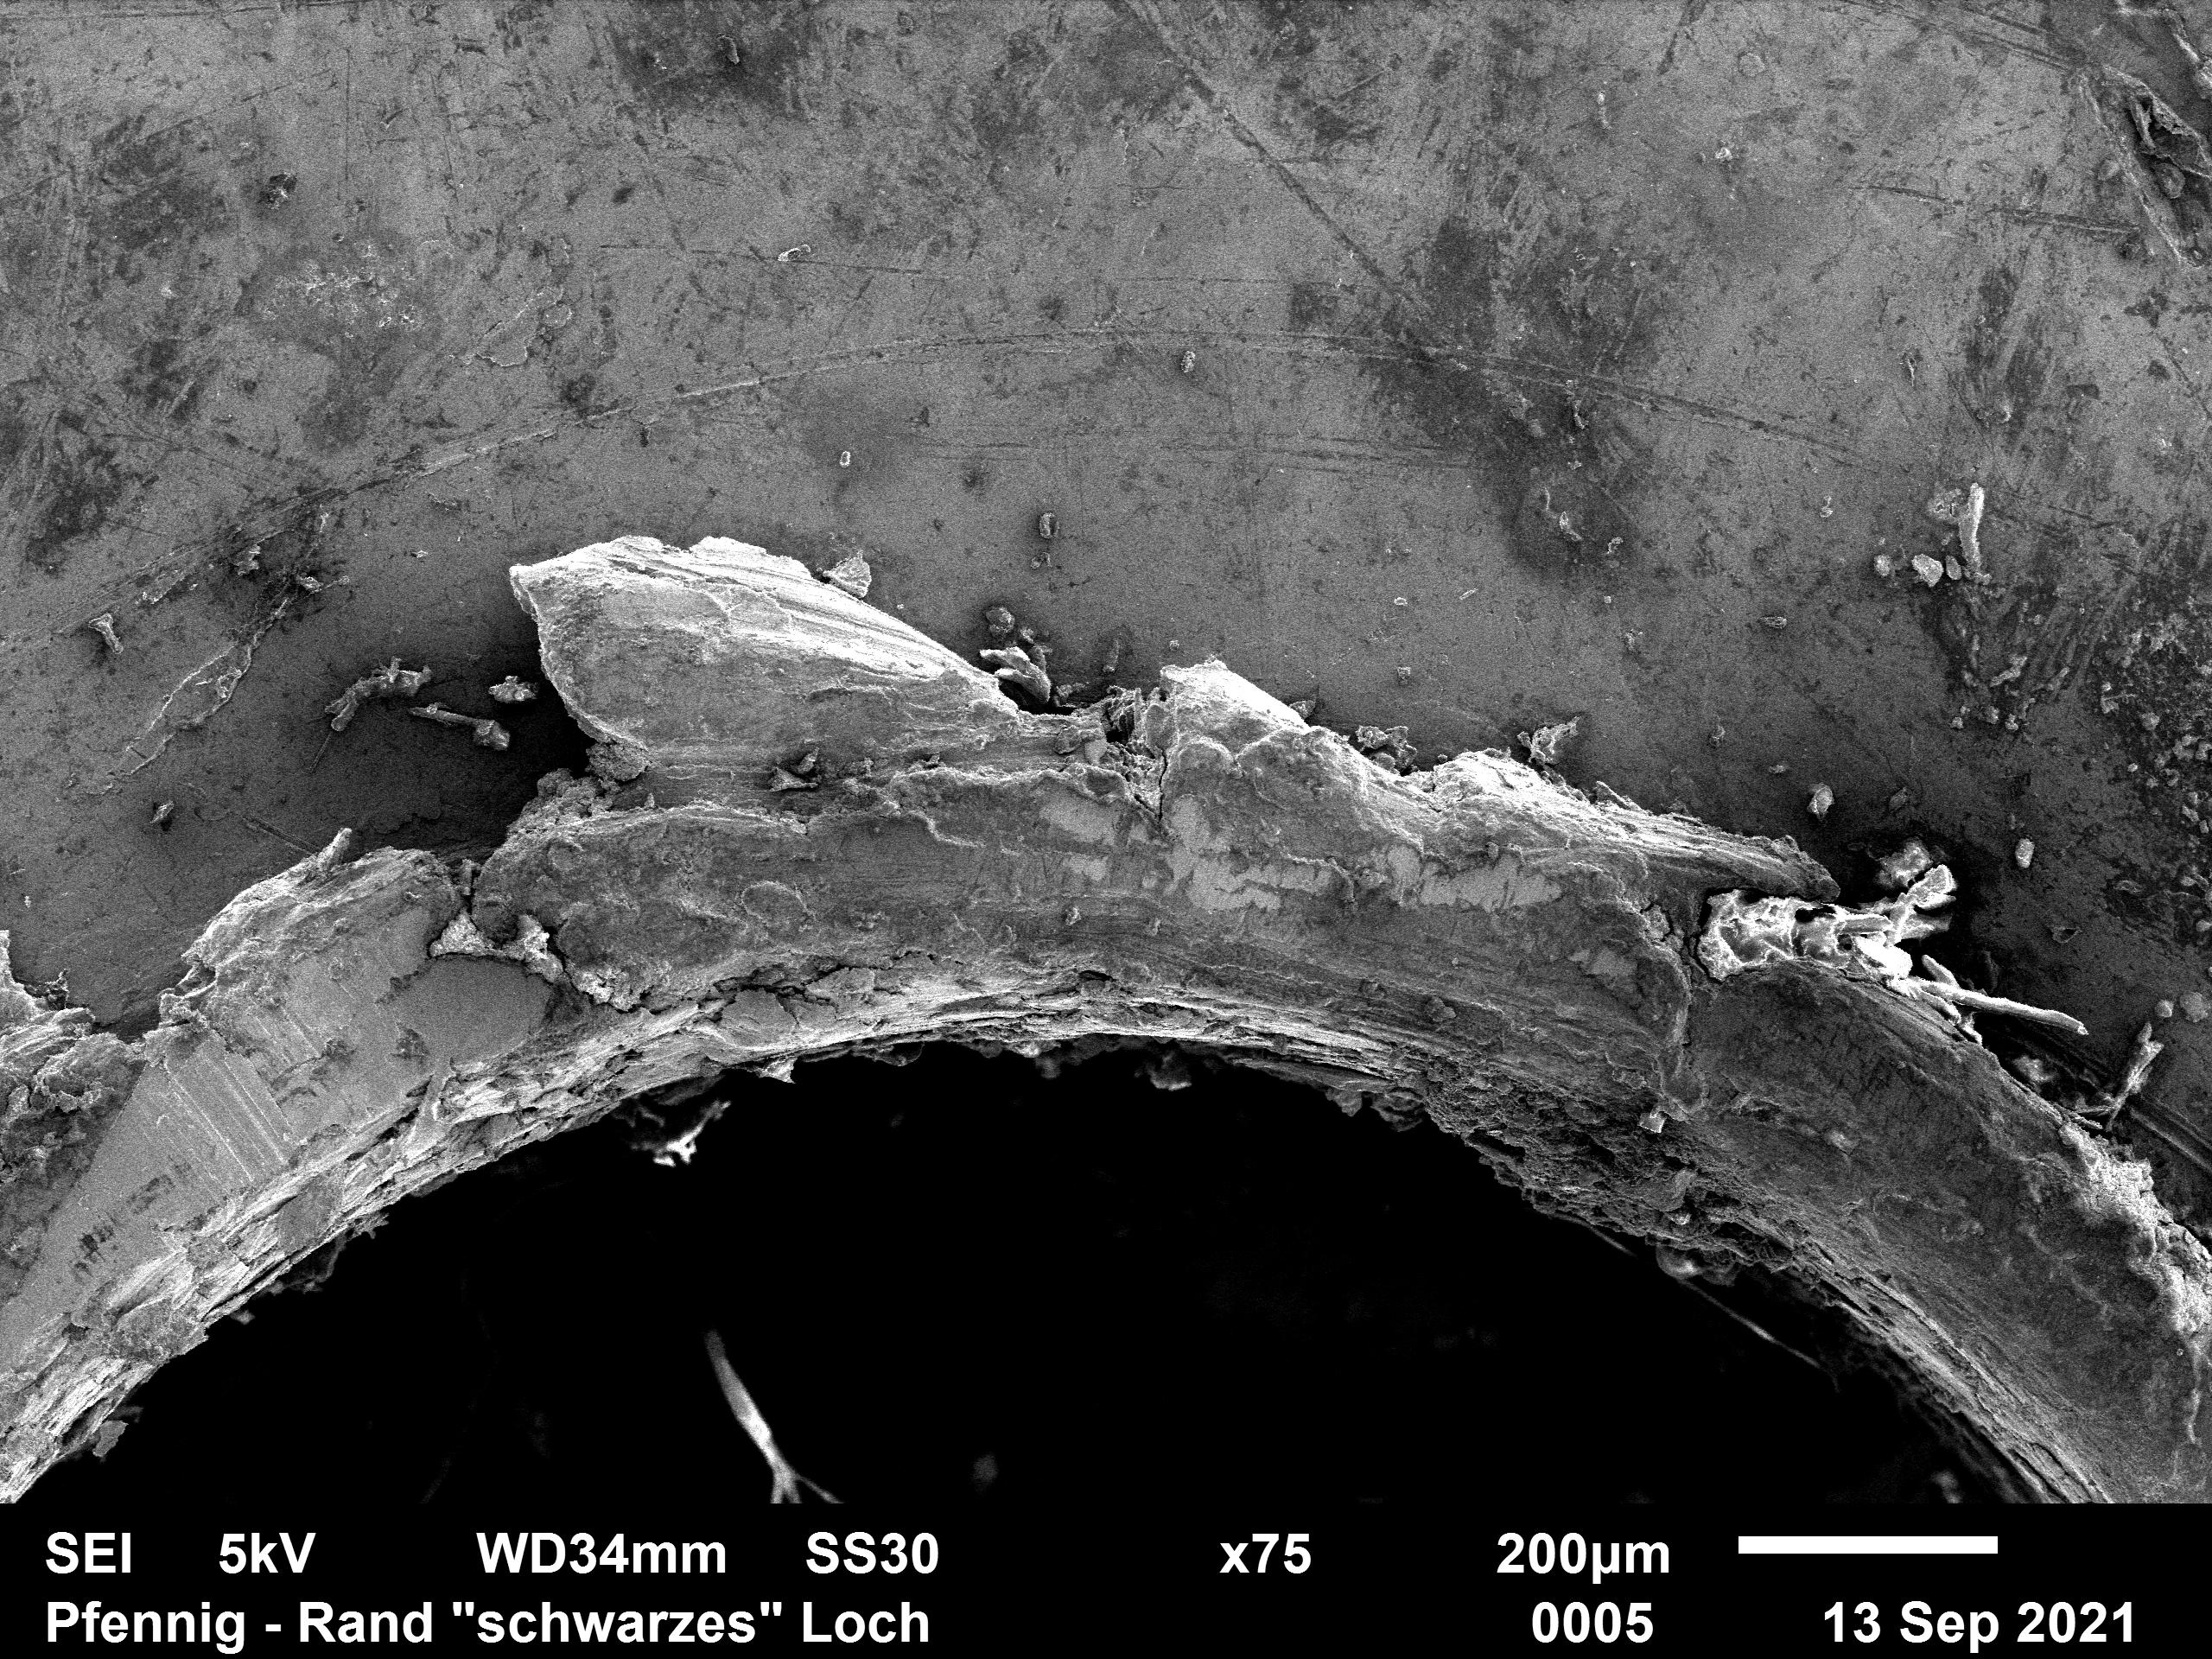
\includegraphics[width=\textwidth]{Auswertung/A/0005.png}
        \caption{$U_B = 5$ kV}
    \end{subfigure}
    \hfill
    \begin{subfigure}[b]{0.45\textwidth}
        \centering
        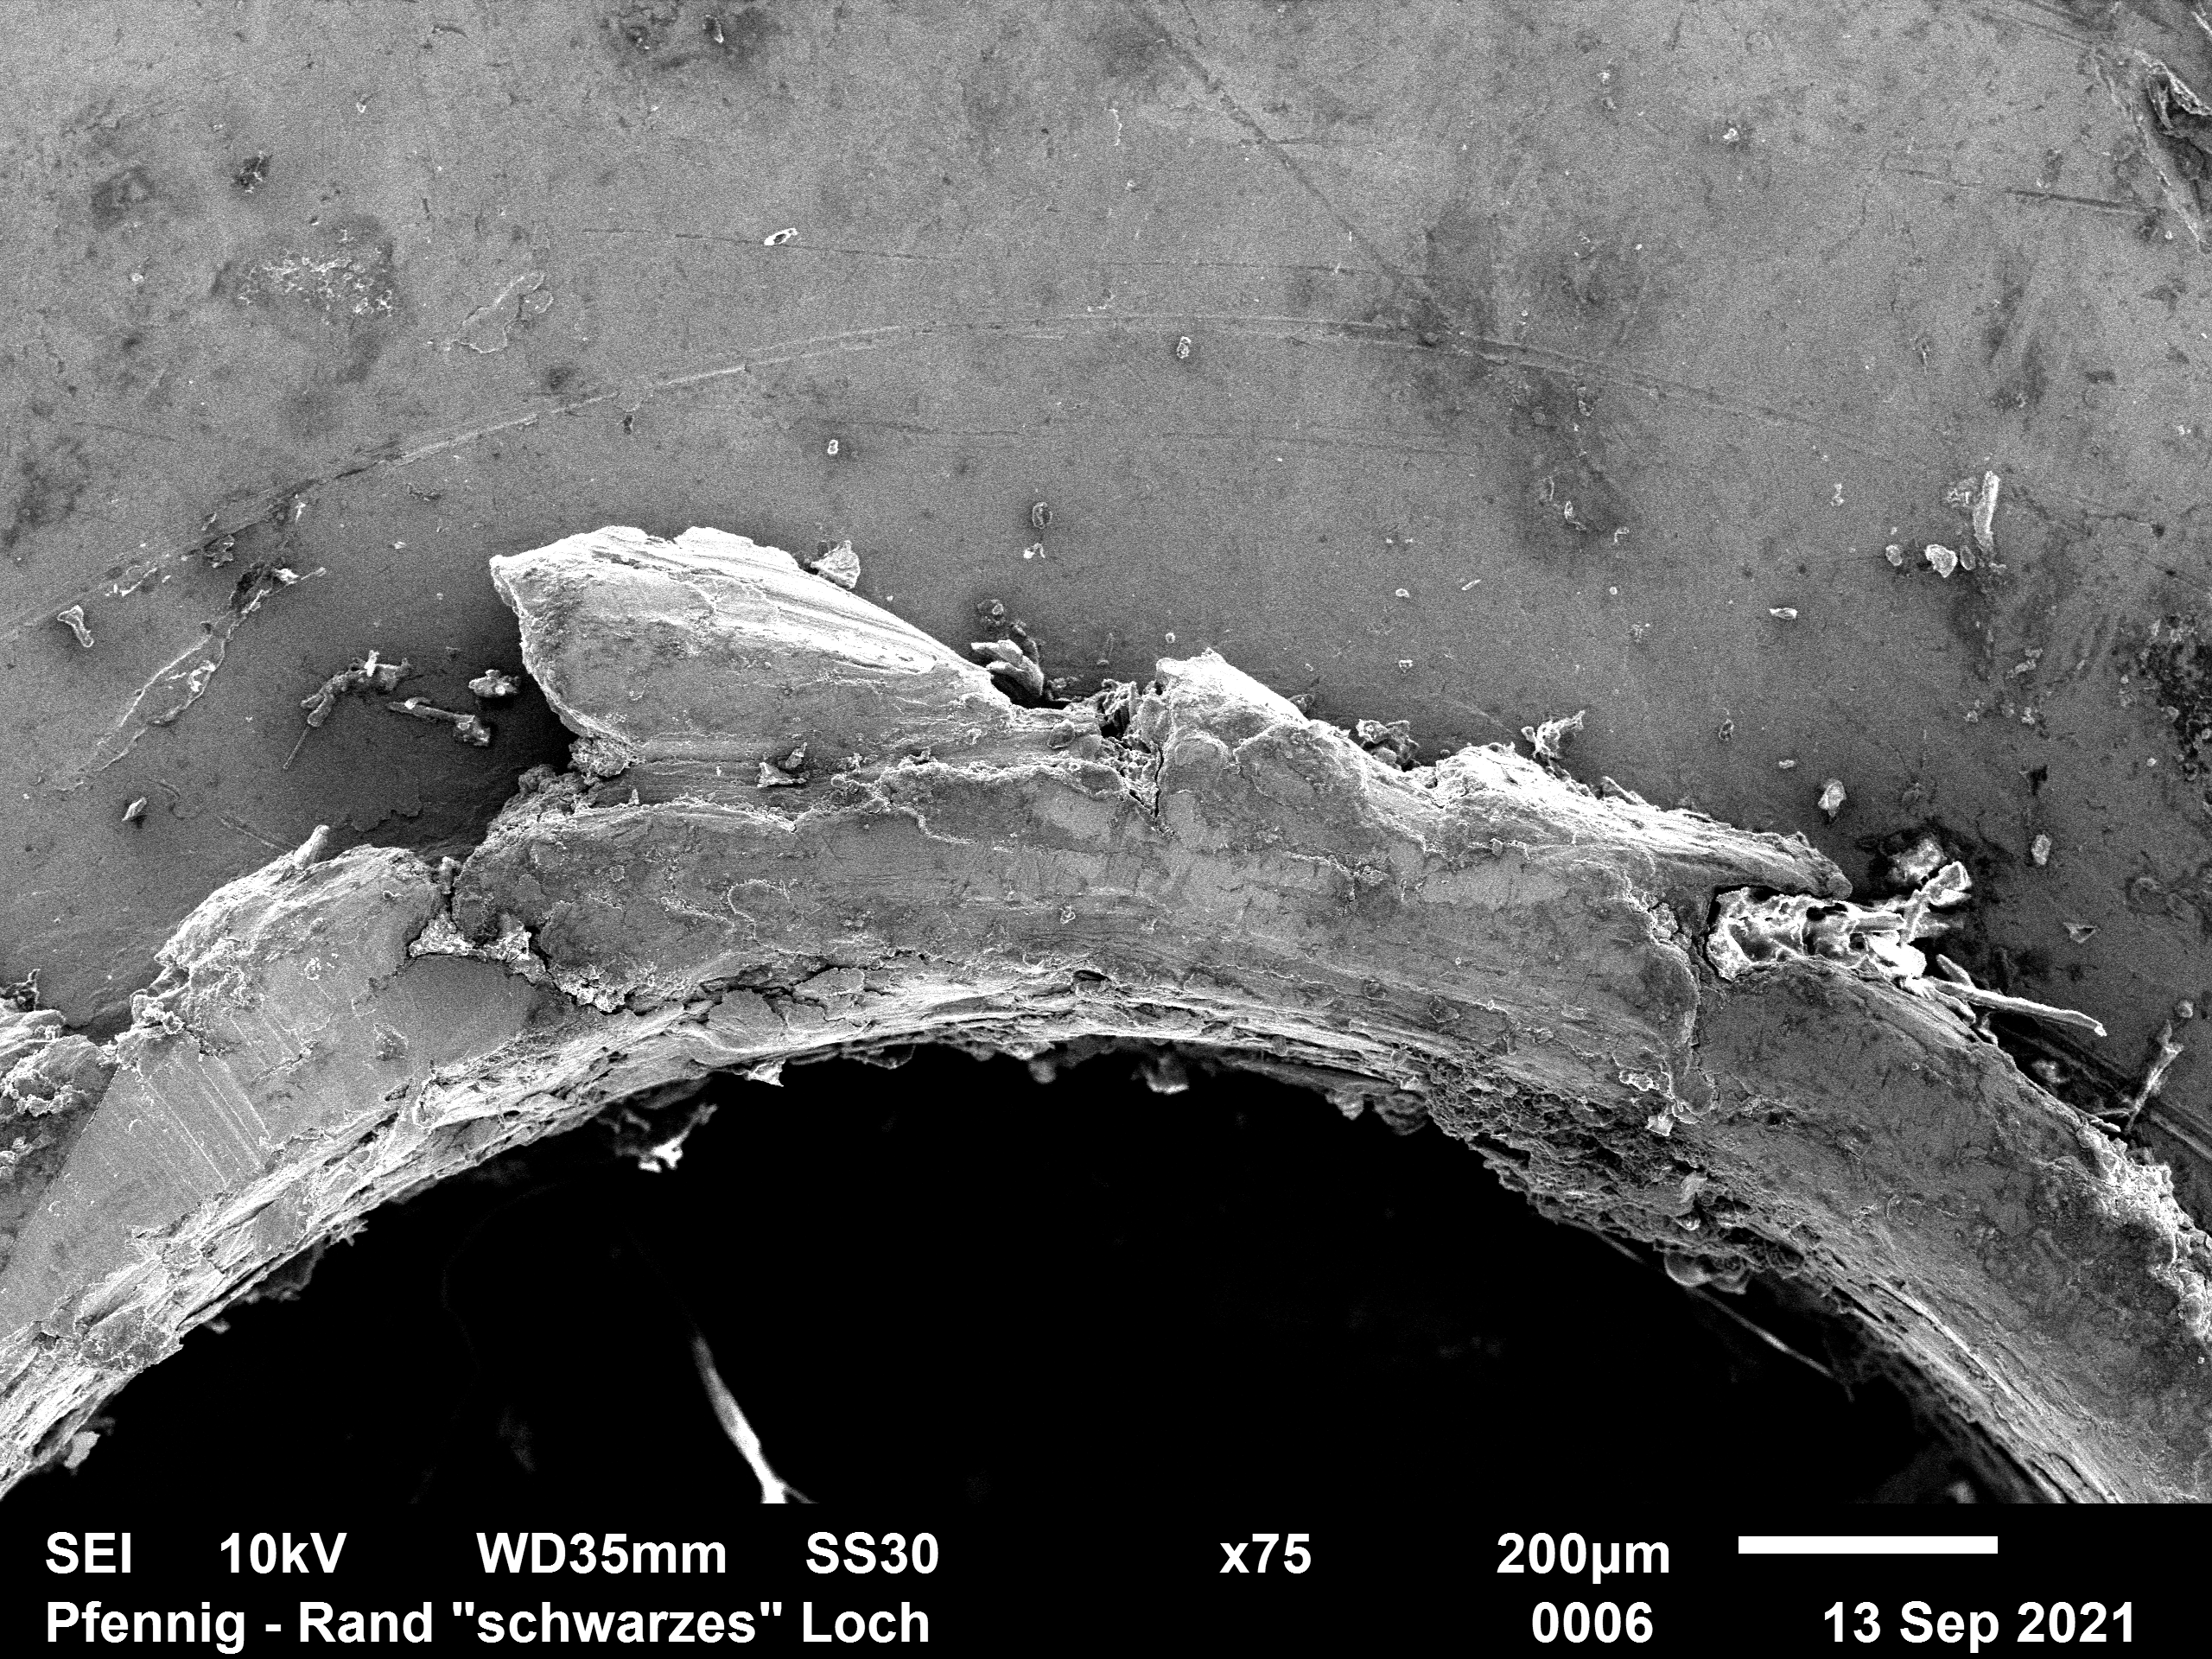
\includegraphics[width=\textwidth]{Auswertung/A/0006.png}
        \caption{$U_B = 10$ kV}
    \end{subfigure}
    \\
    \begin{subfigure}[b]{0.45\textwidth}
        \centering
        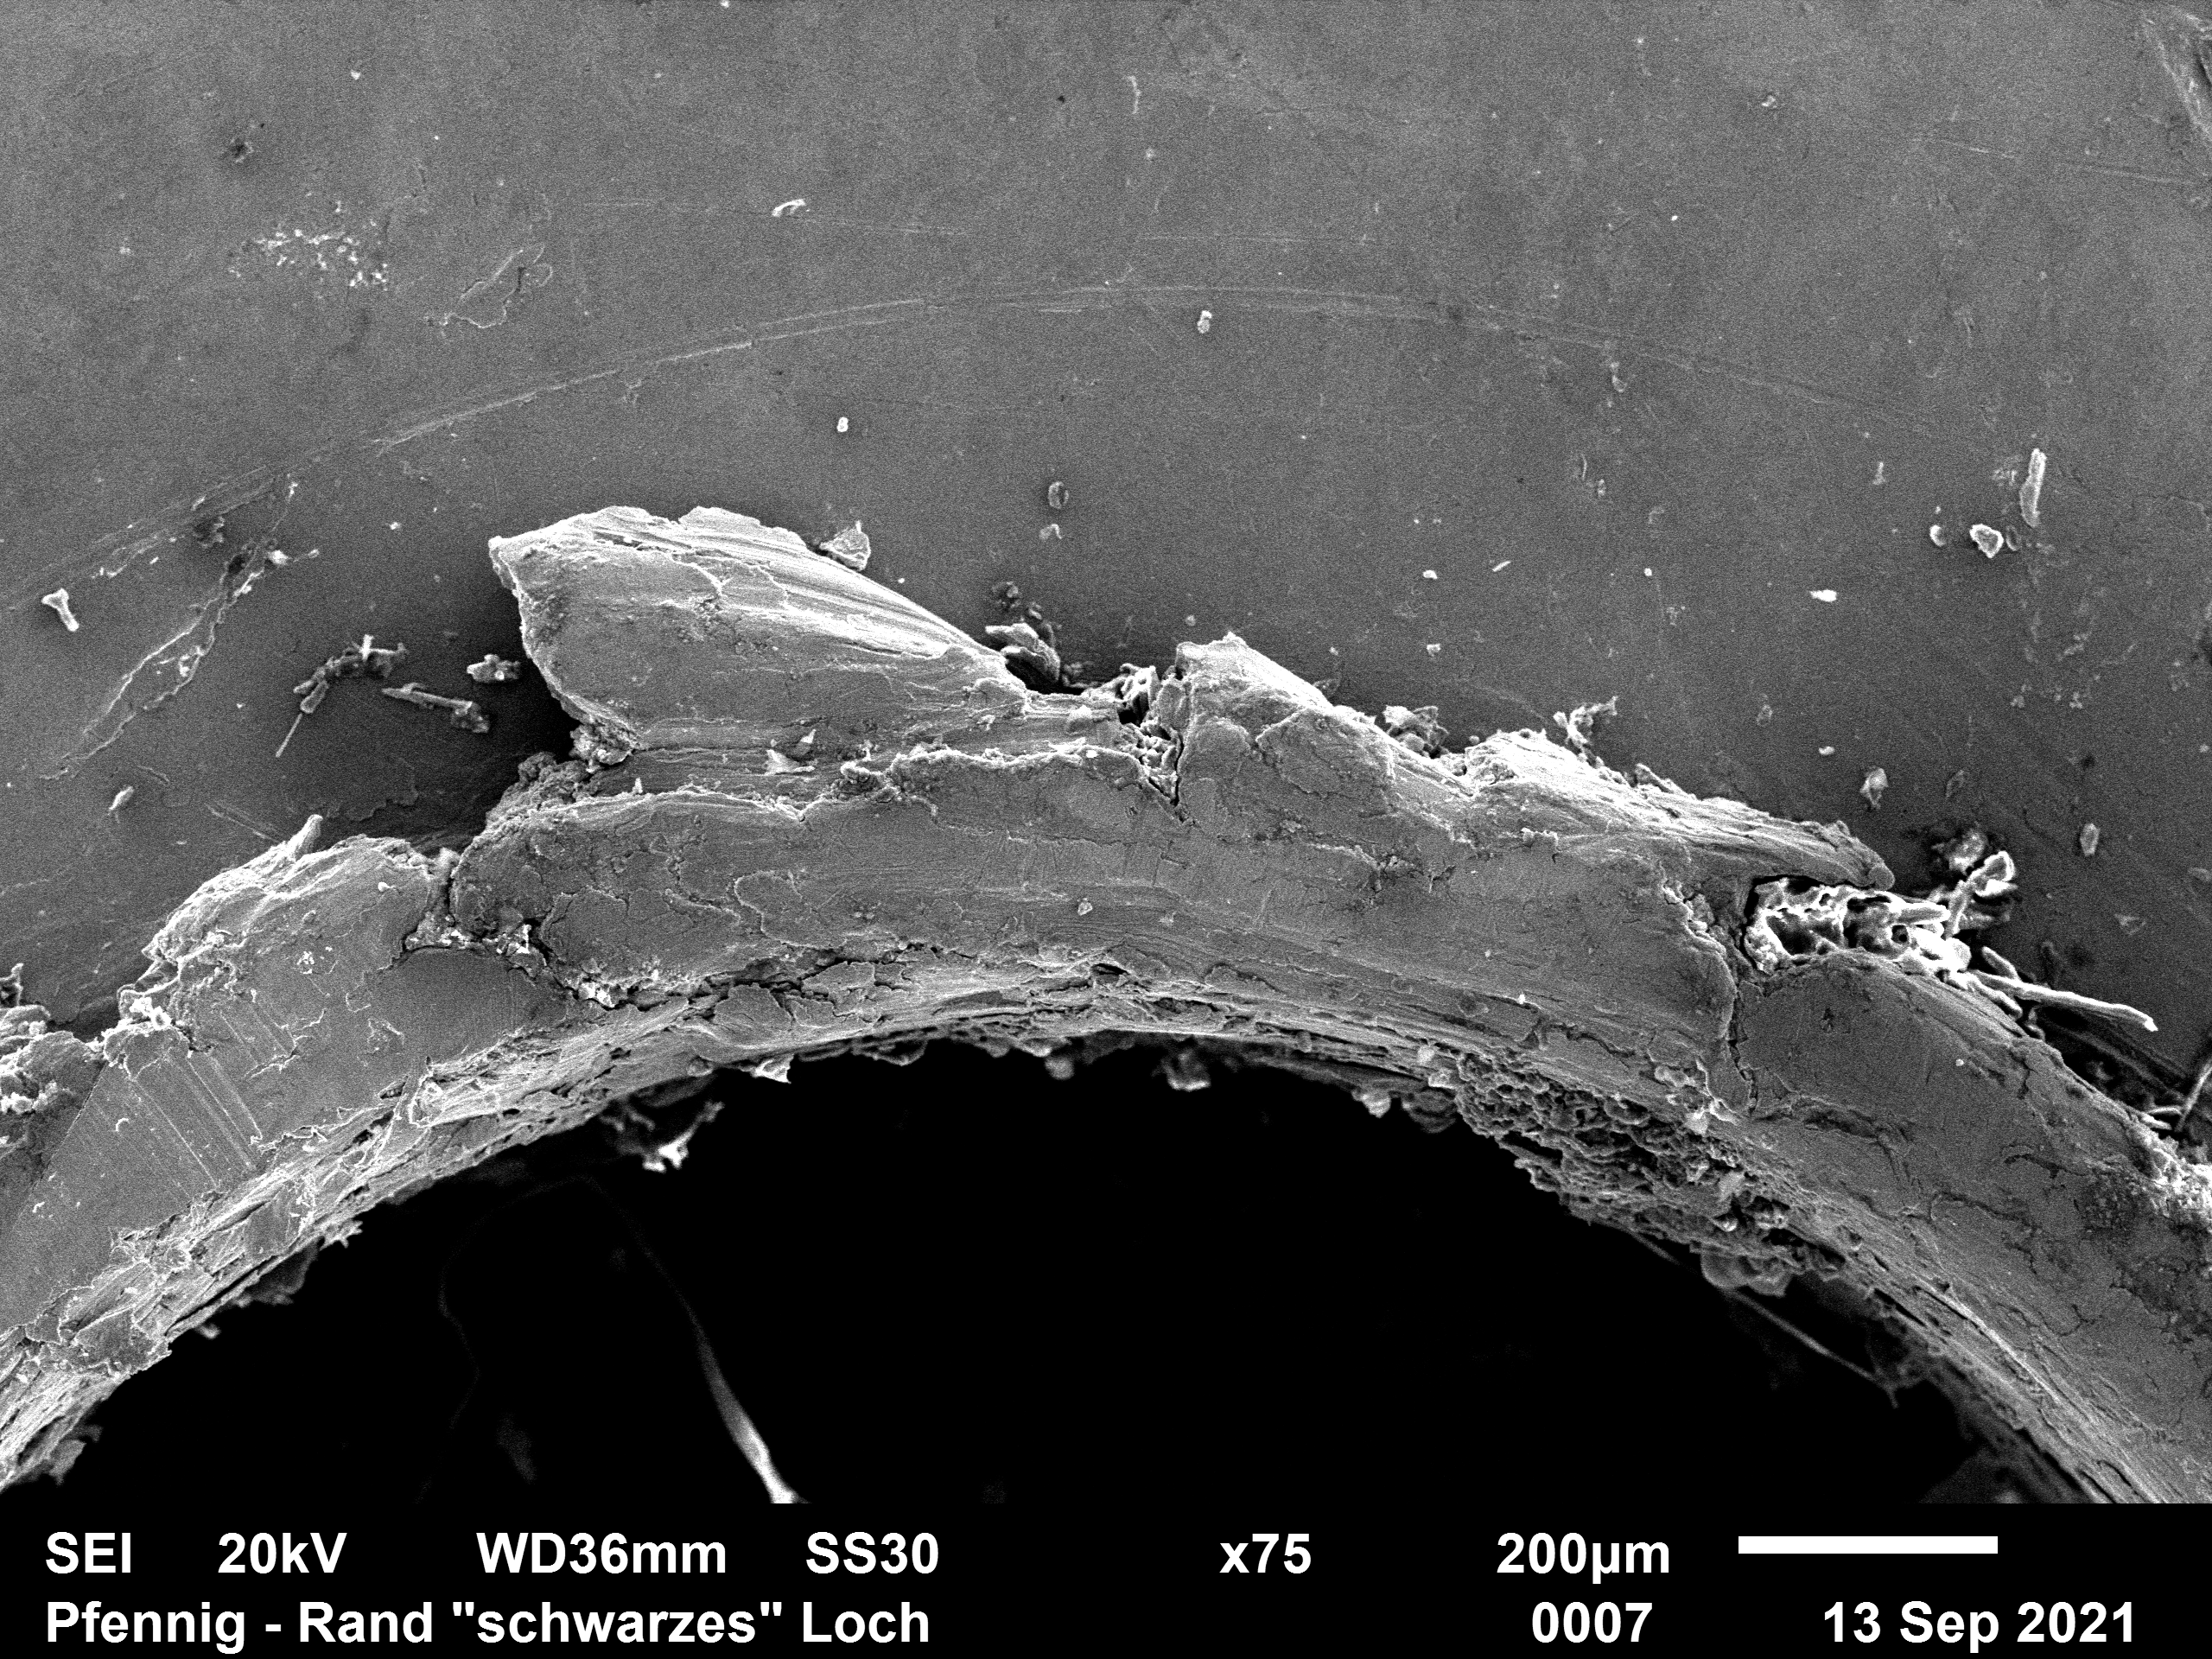
\includegraphics[width=\textwidth]{Auswertung/A/0007.png}
        \caption{$U_B = 20$ kV}
    \end{subfigure}
    \hfill
    \begin{subfigure}[b]{0.45\textwidth}
        \centering
        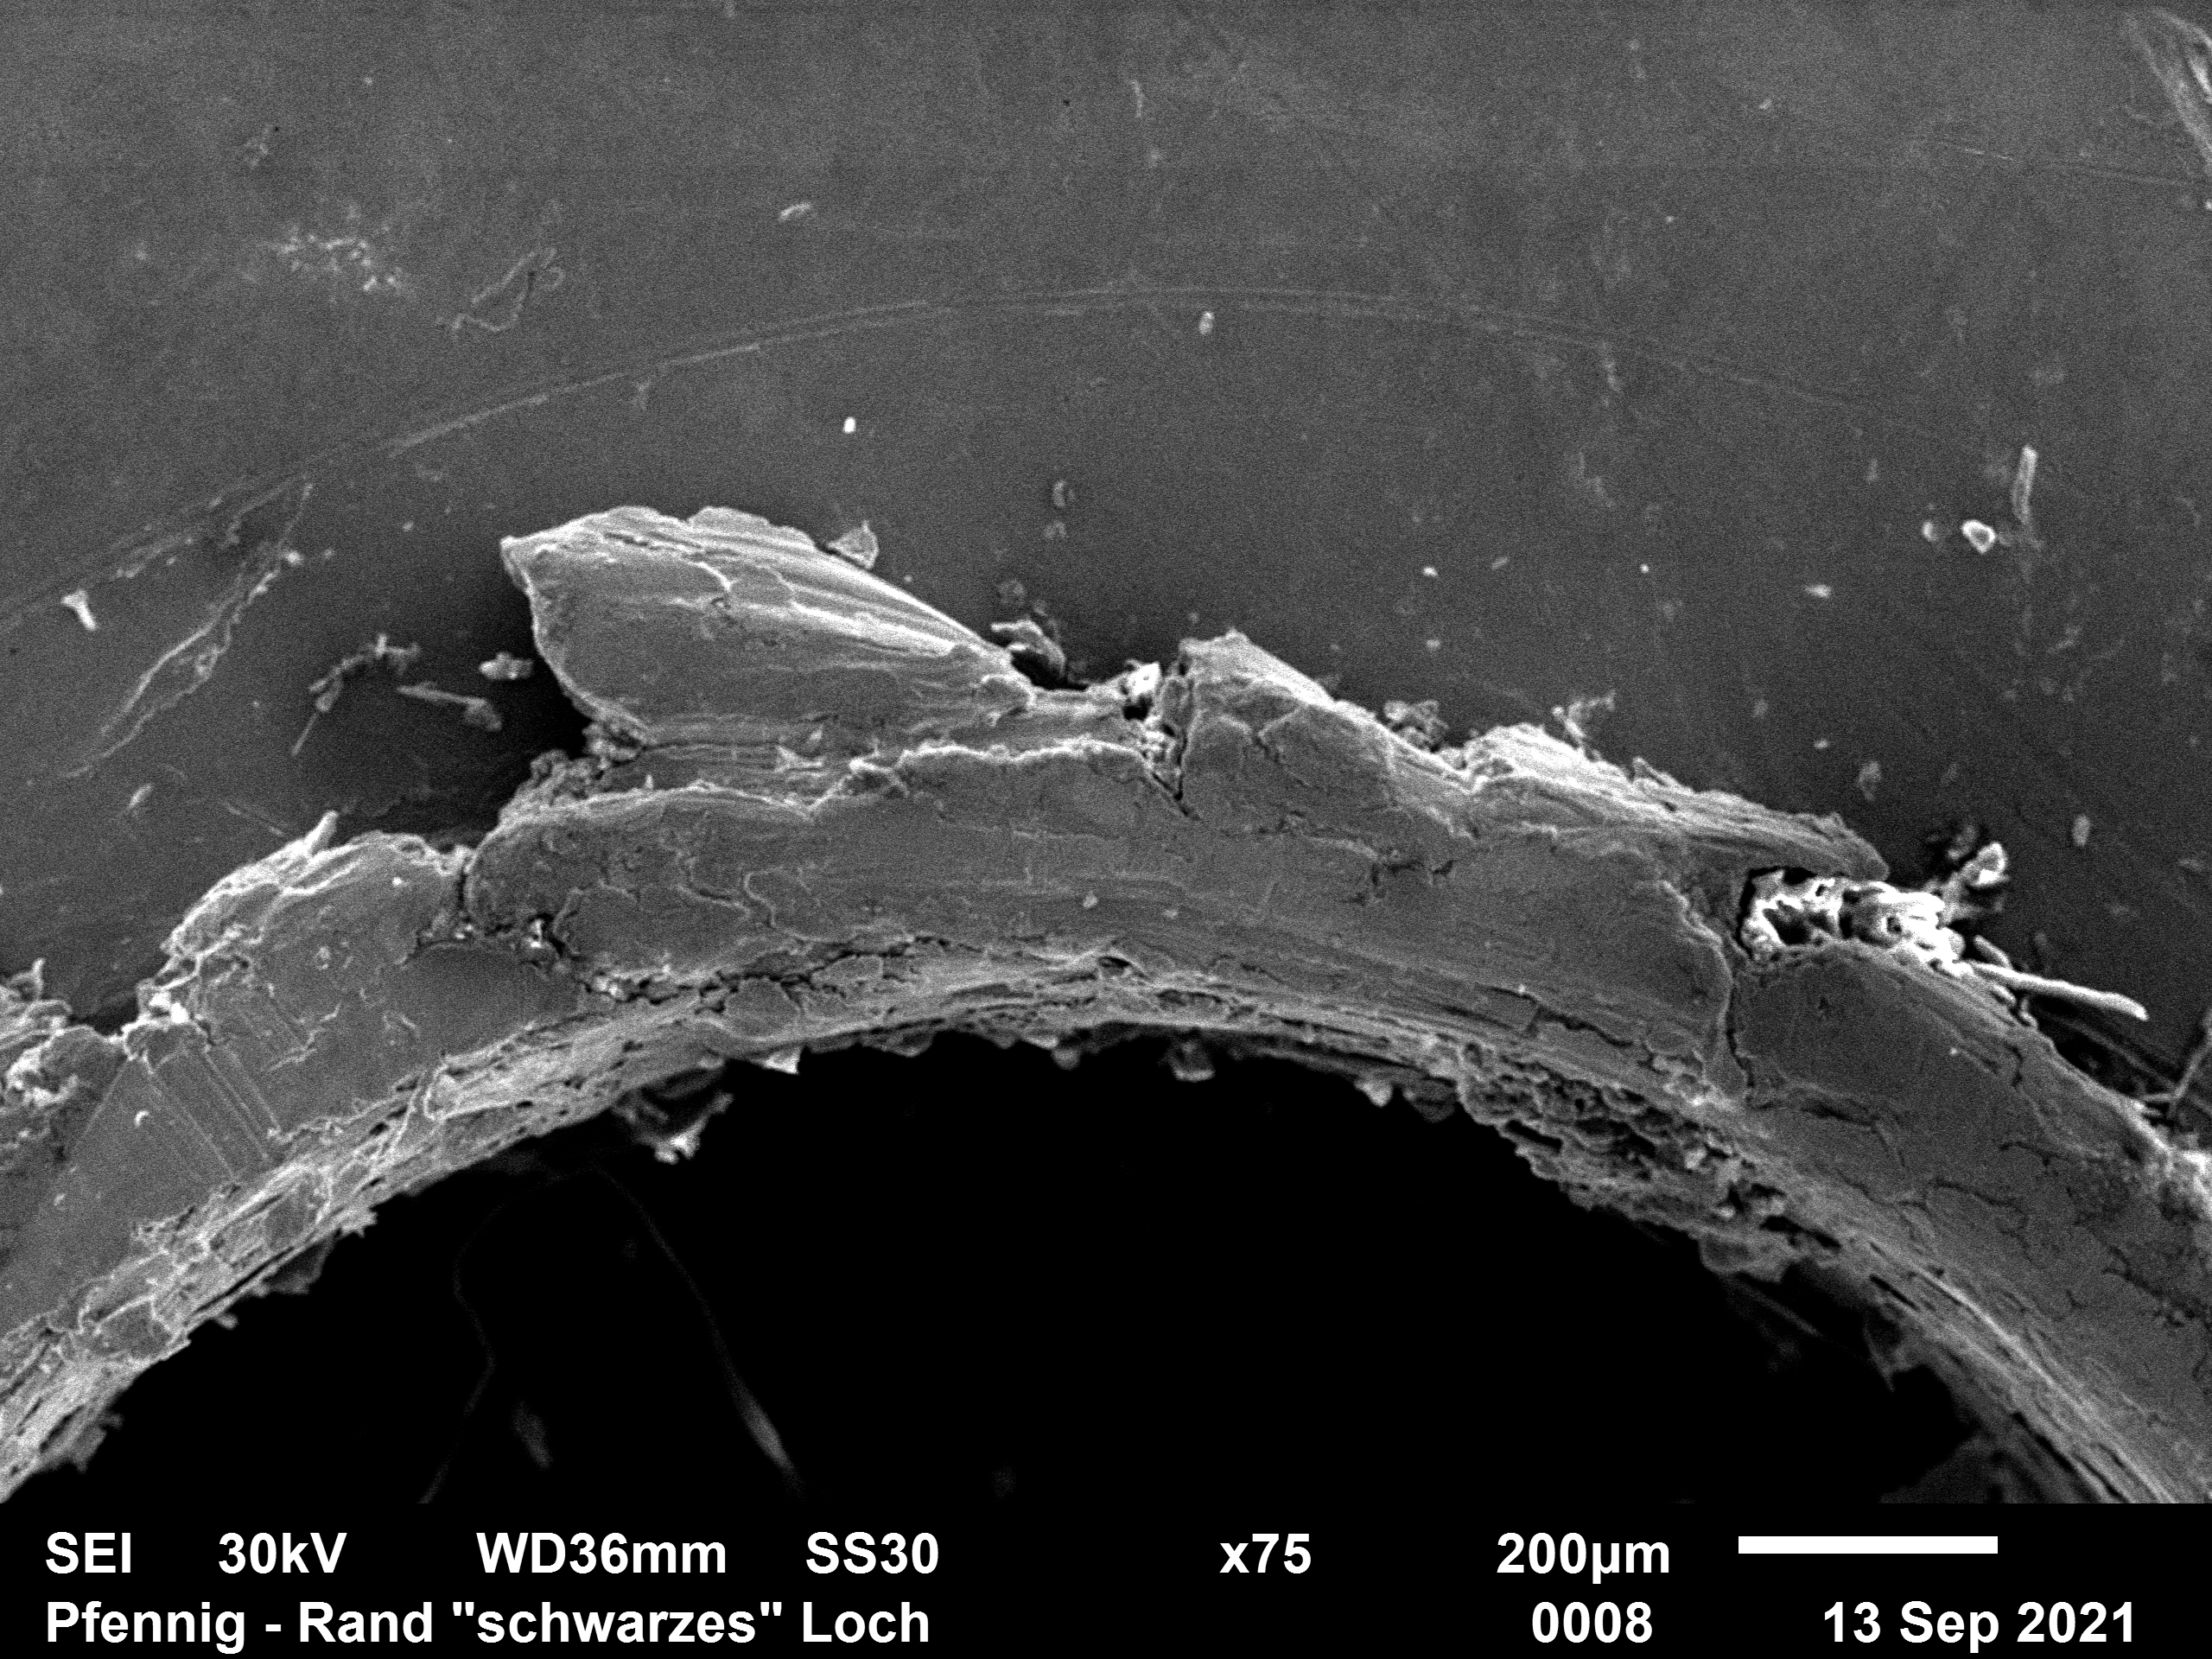
\includegraphics[width=\textwidth]{Auswertung/A/0008.png}
        \caption{$U_B = 30$ kV}
    \end{subfigure}
    \caption{SEI bei unterschiedlichen Beschleunigunsspannungen}
\end{figure}

Disskussion!

\newpage
Als Nächstes wurde der Everhart-Thronley-Detektor im RE Modus (REF) verwendet und dabei ebenfalls die Beschleunigungsspannung variiert.
\begin{figure}[h]
    \centering
    
    \begin{subfigure}[b]{0.45\textwidth}
        \centering
        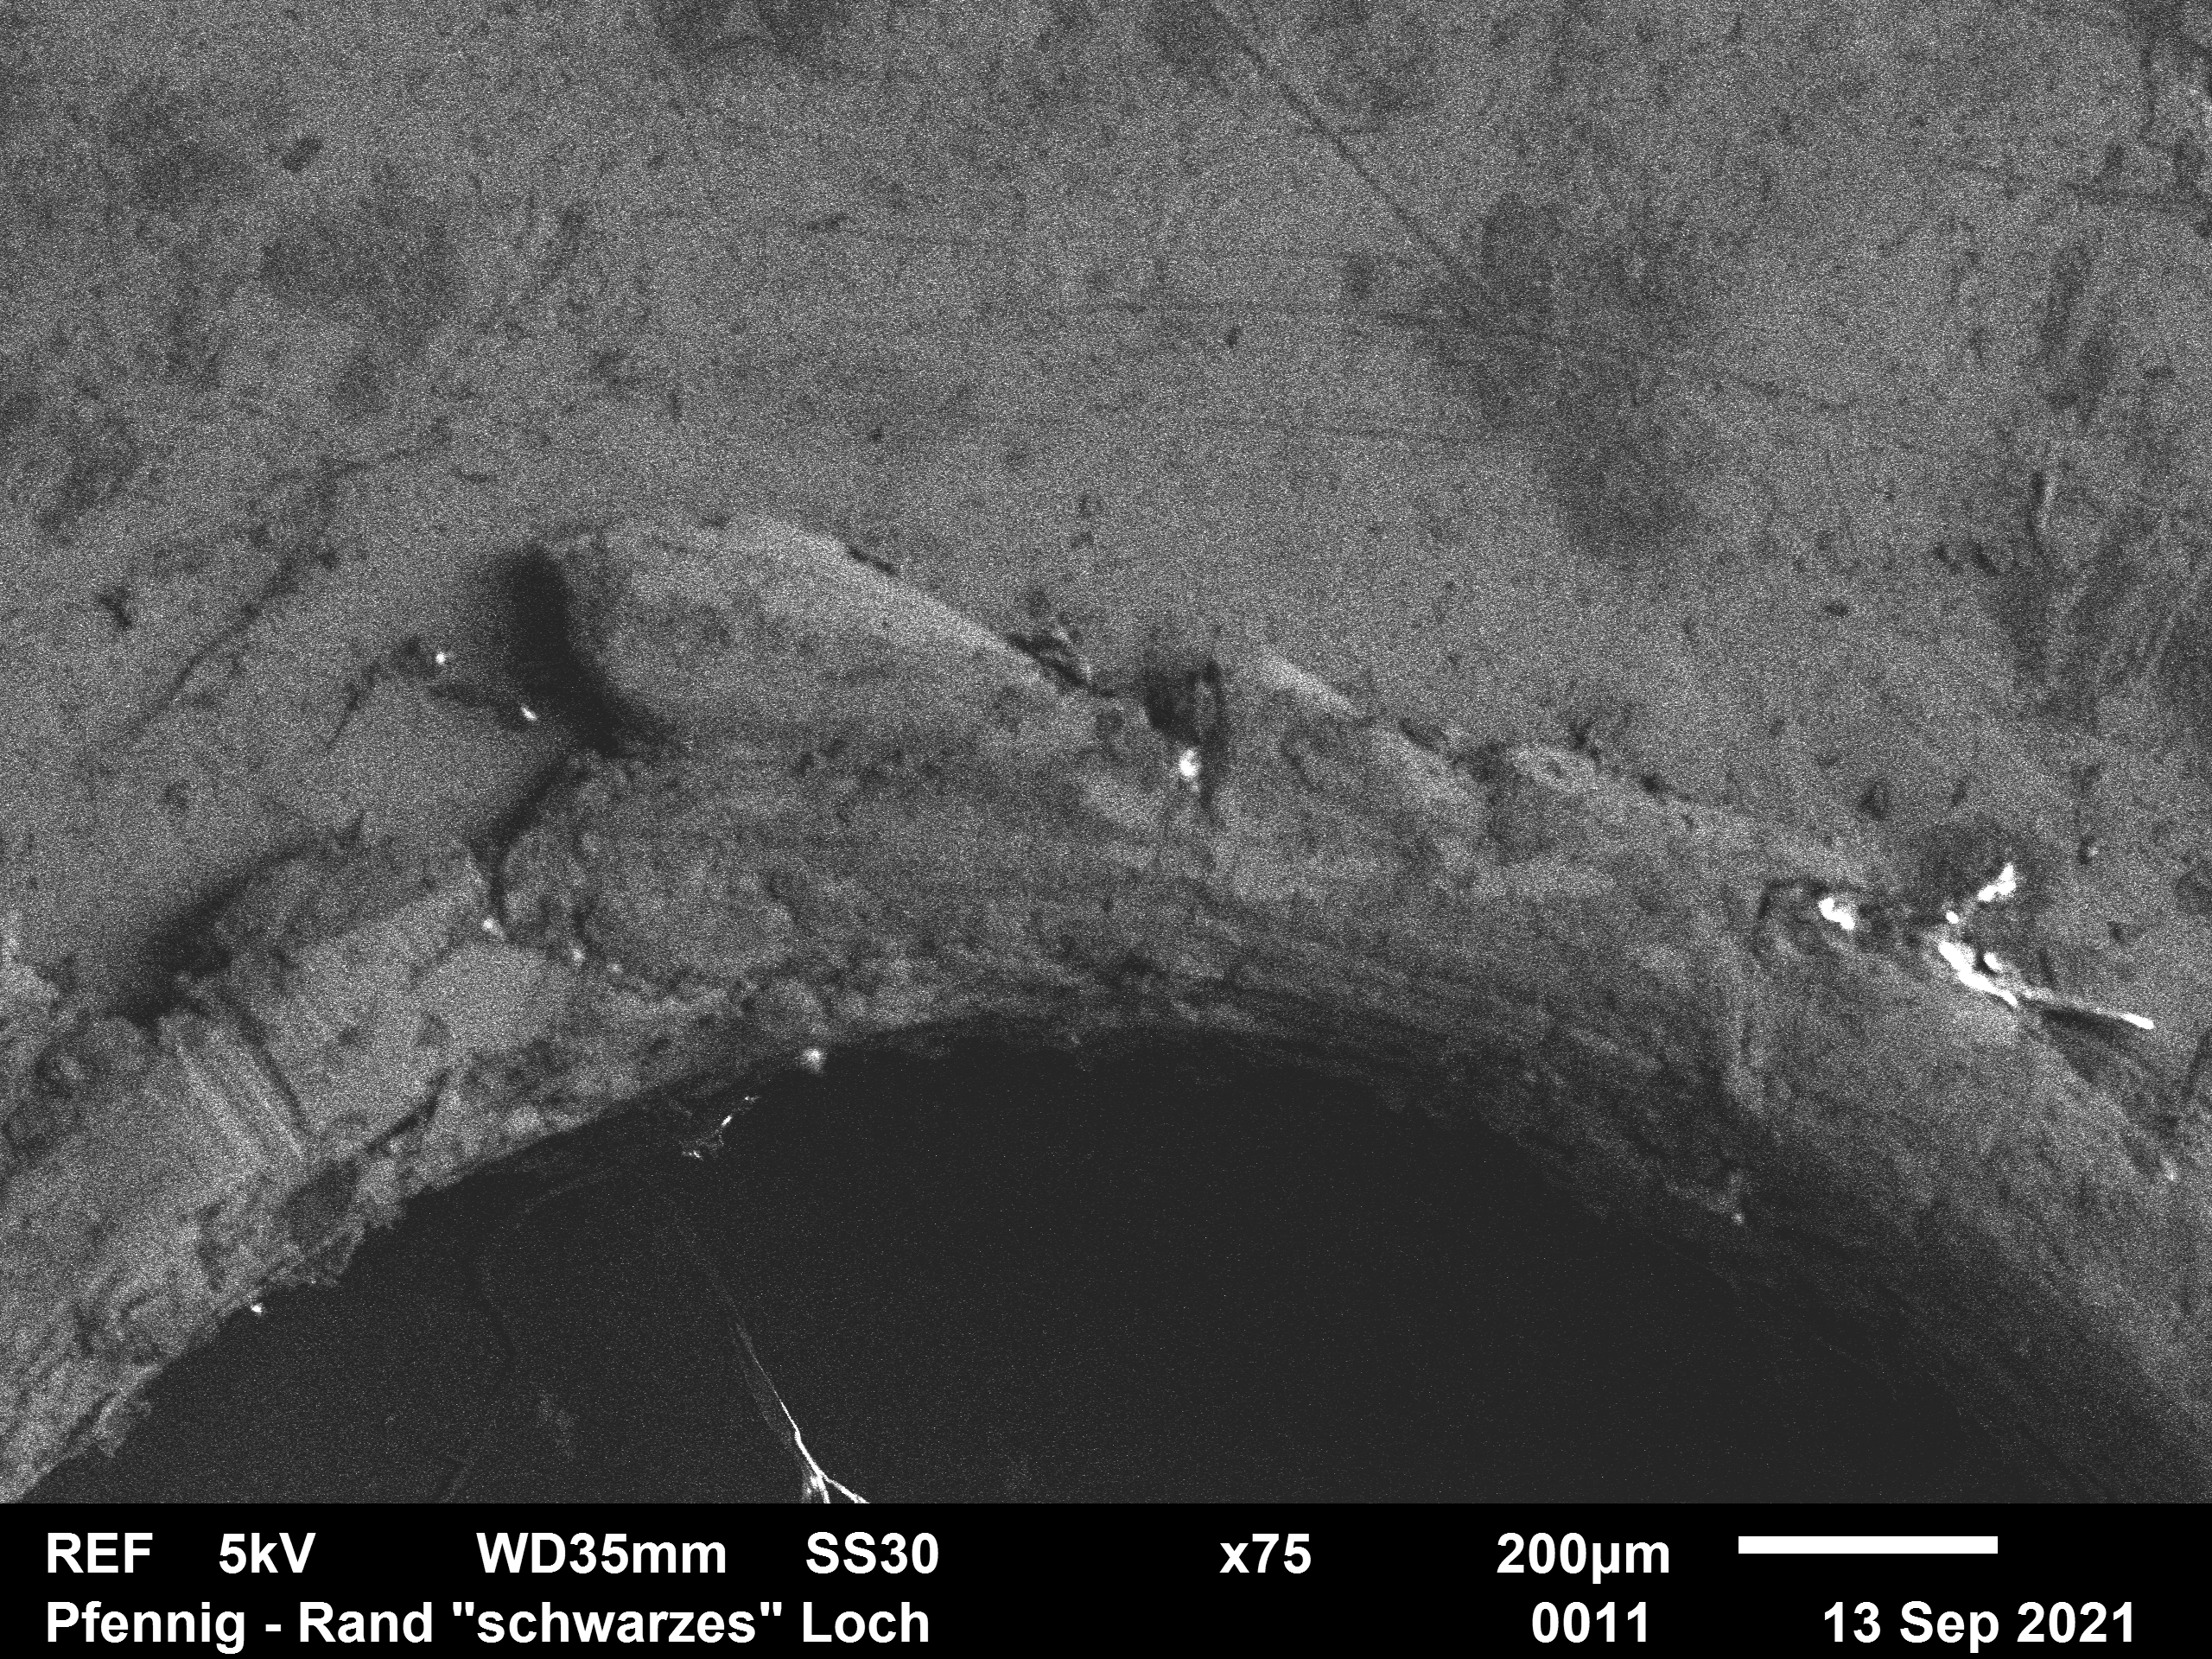
\includegraphics[width=\textwidth]{Auswertung/A/0011.png}
        \caption{$U_B = 5$ kV}
    \end{subfigure}
    \hfill
    \begin{subfigure}[b]{0.45\textwidth}
        \centering
        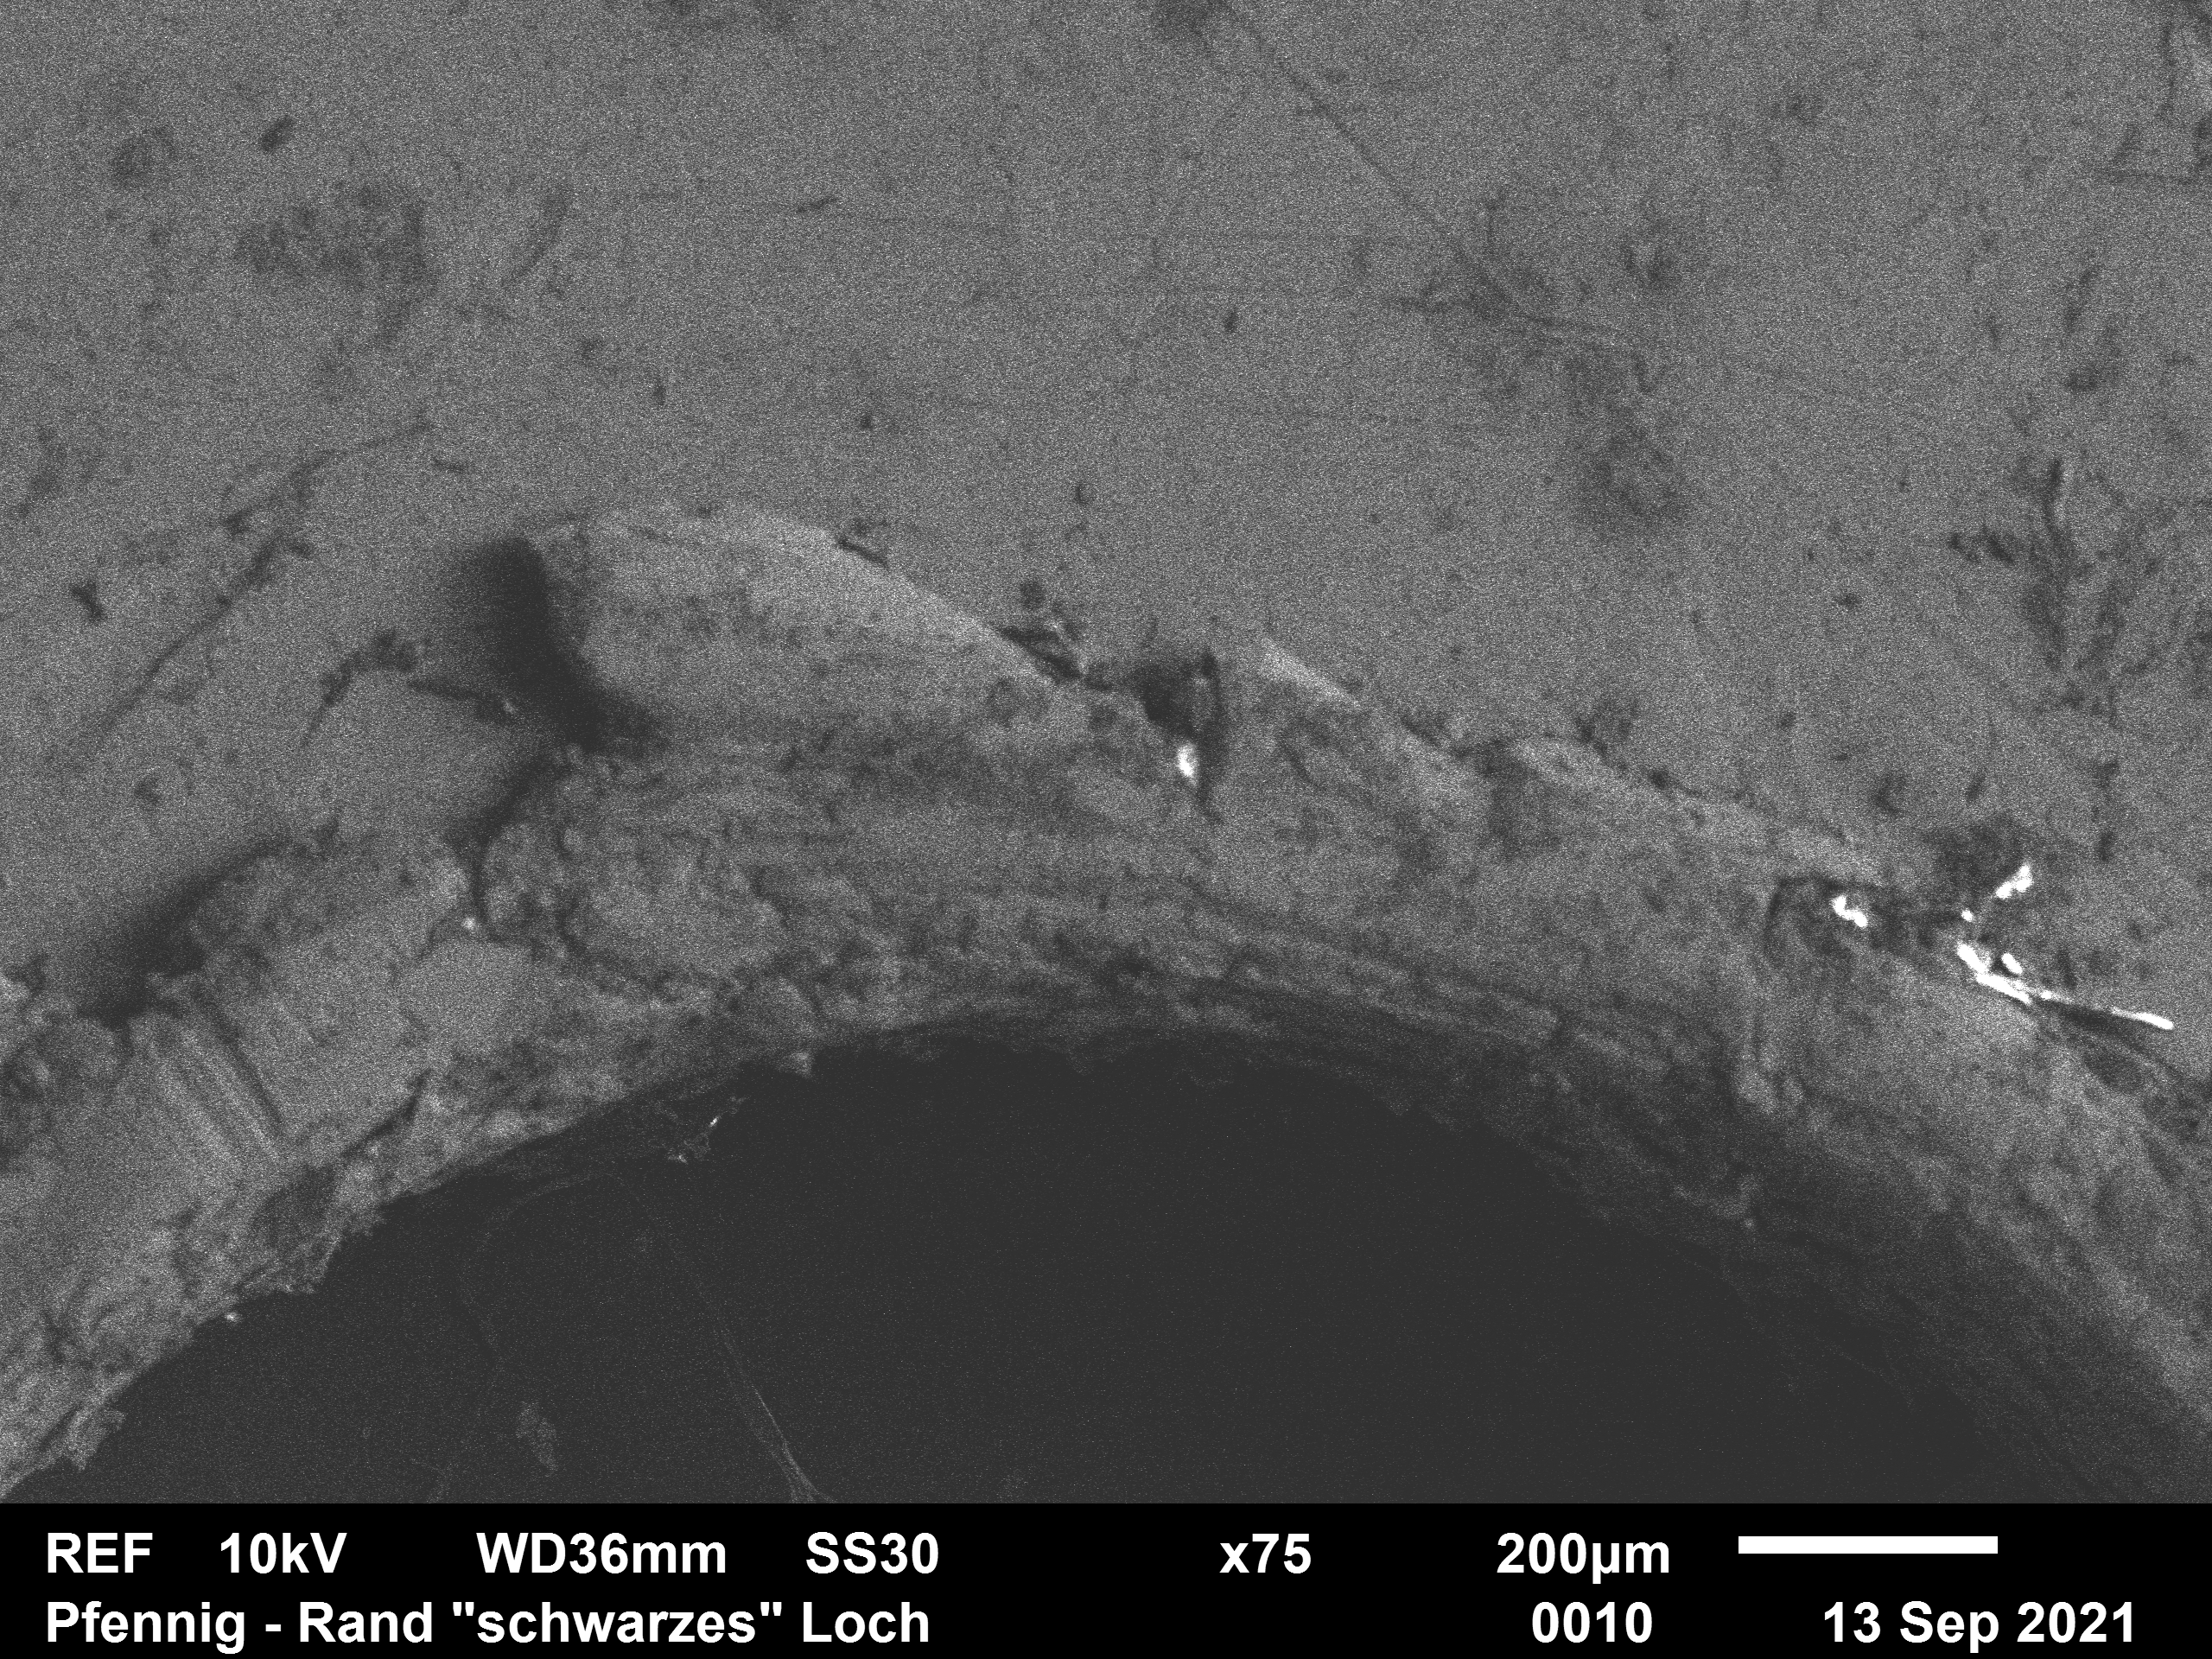
\includegraphics[width=\textwidth]{Auswertung/A/0010.png}
        \caption{$U_B = 10$ kV}
    \end{subfigure}
    \\
    \begin{subfigure}[b]{0.45\textwidth}
        \centering
        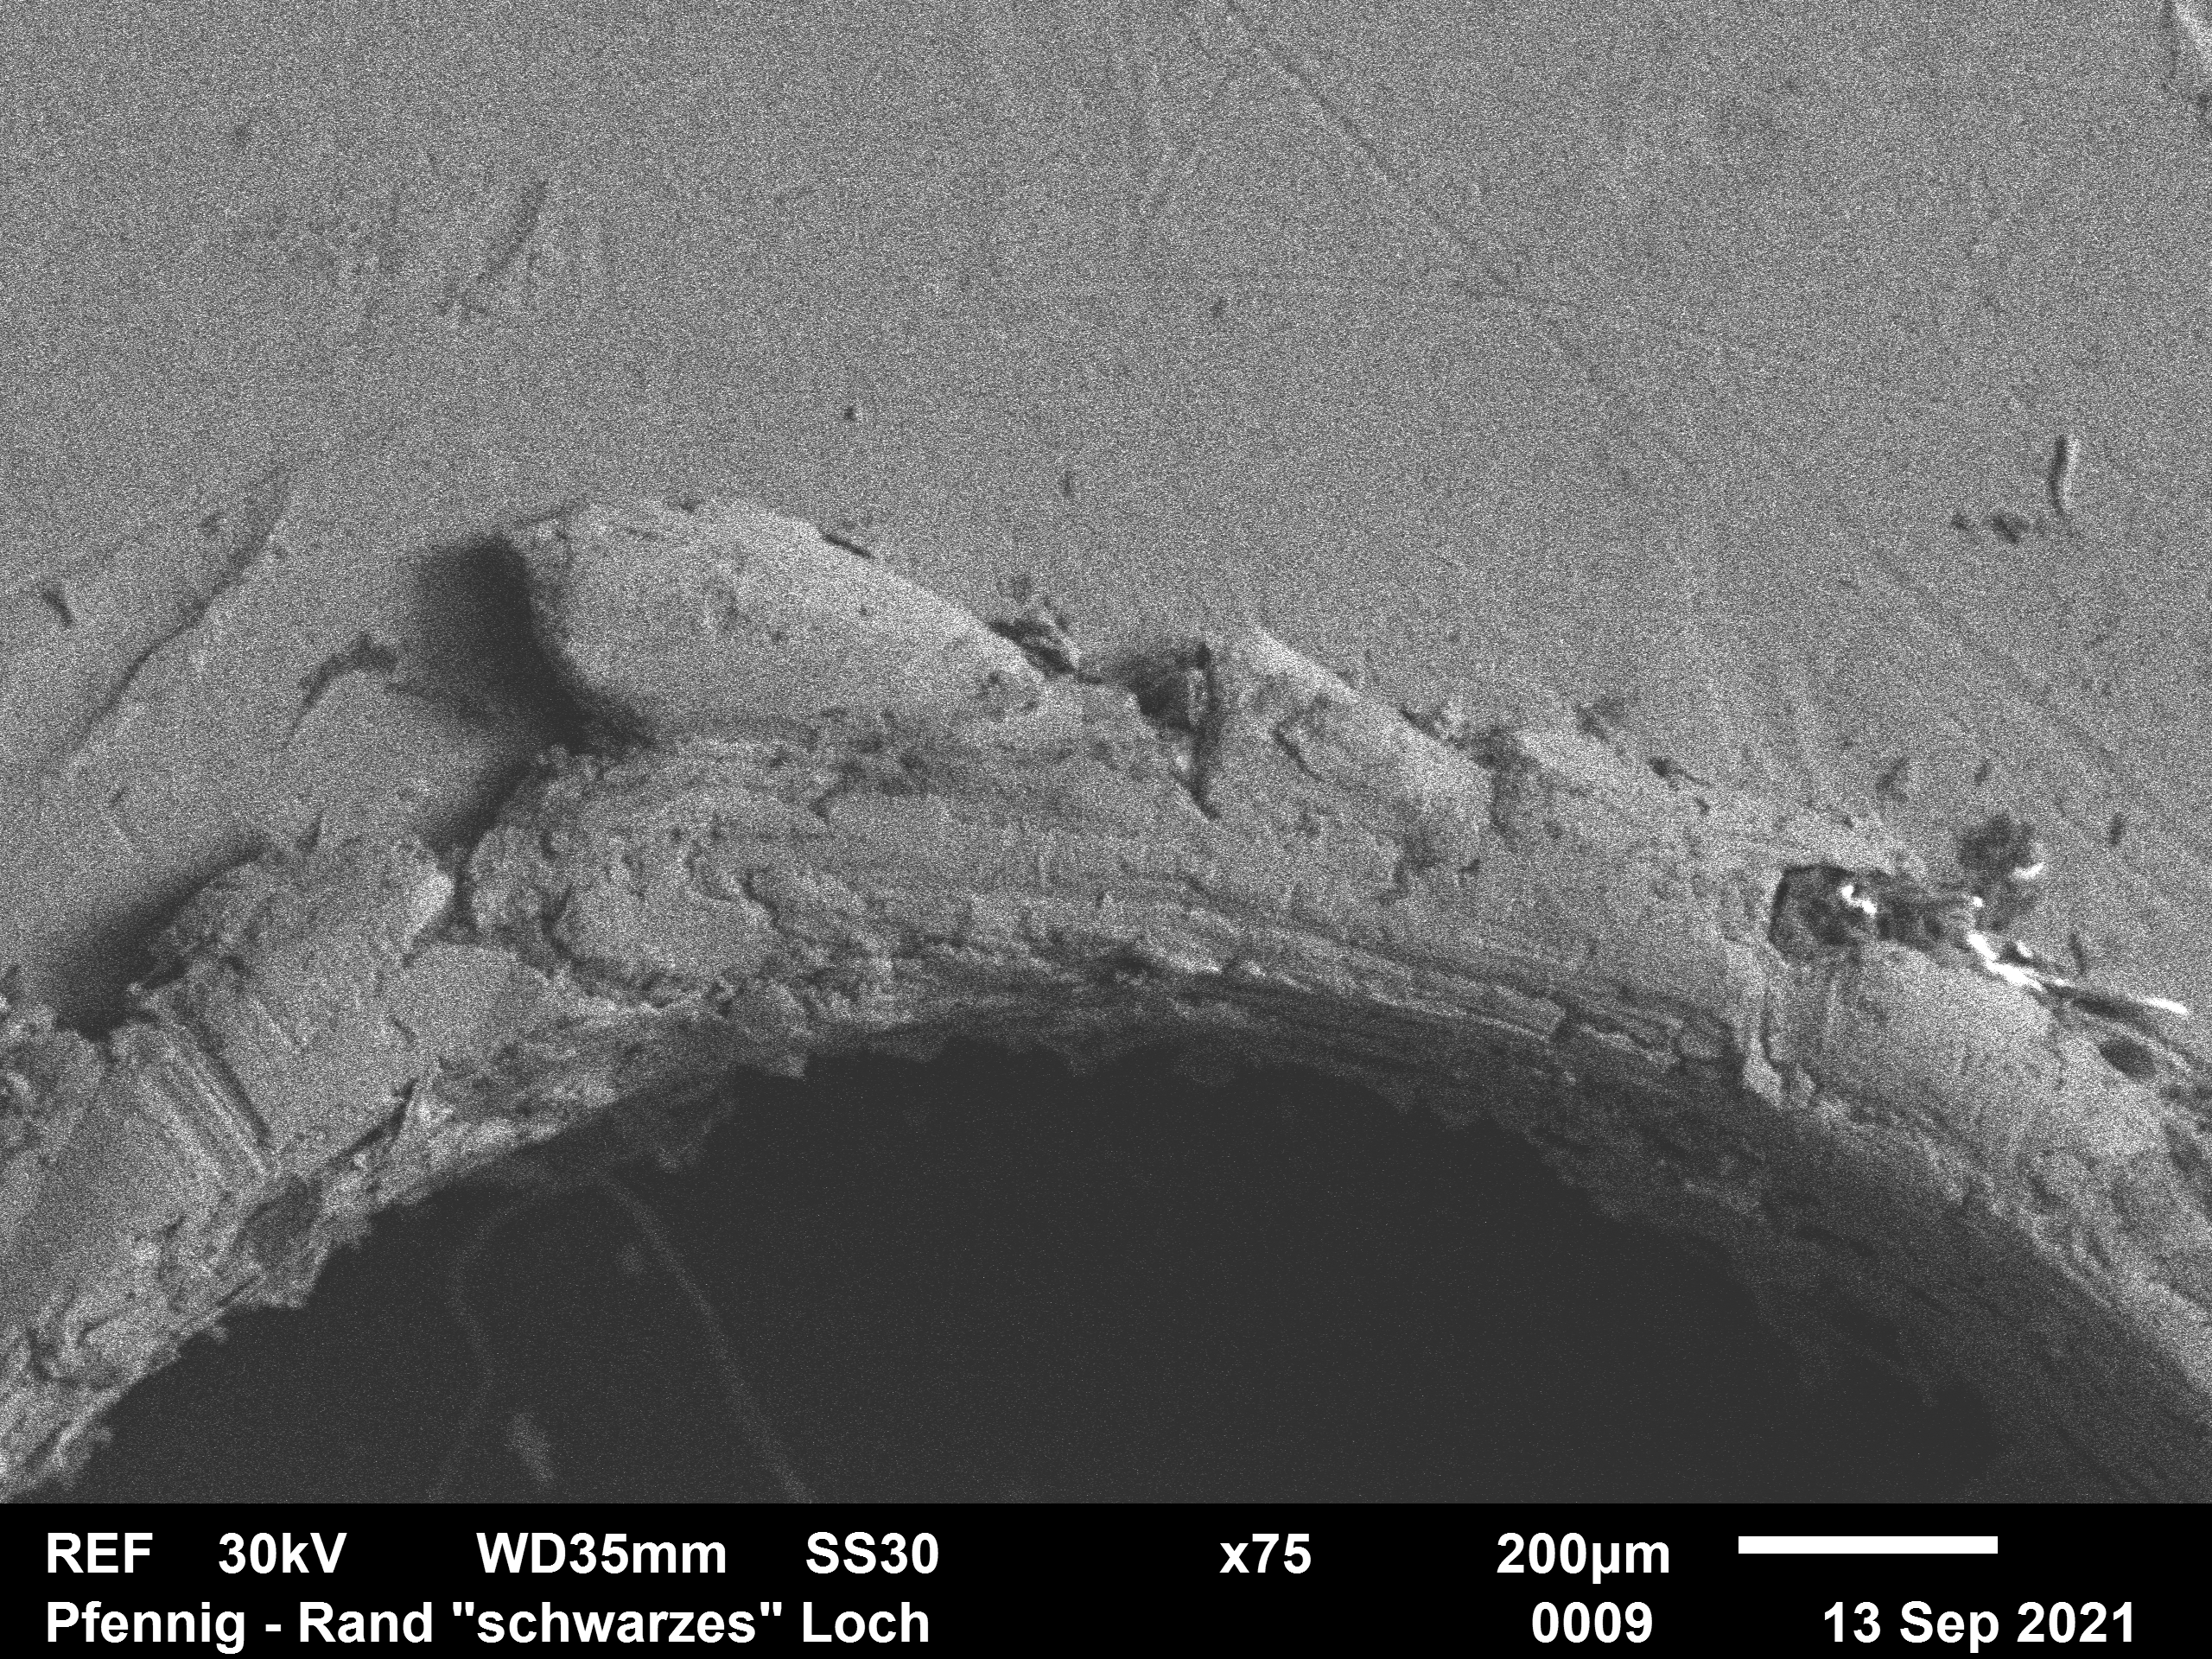
\includegraphics[width=\textwidth]{Auswertung/A/0009.png}
        \caption{$U_B = 30$ kV}
    \end{subfigure}
    \caption{REF bei unterschiedlichen Beschleunigunsspannungen}
\end{figure}

Diskussion!

\newpage
Das gleich wurde auch für den Halbleiterdetektor im Compo-Mode (BEC) gemacht.
\begin{figure}[h]
    \centering
    
    \begin{subfigure}[b]{0.45\textwidth}
        \centering
        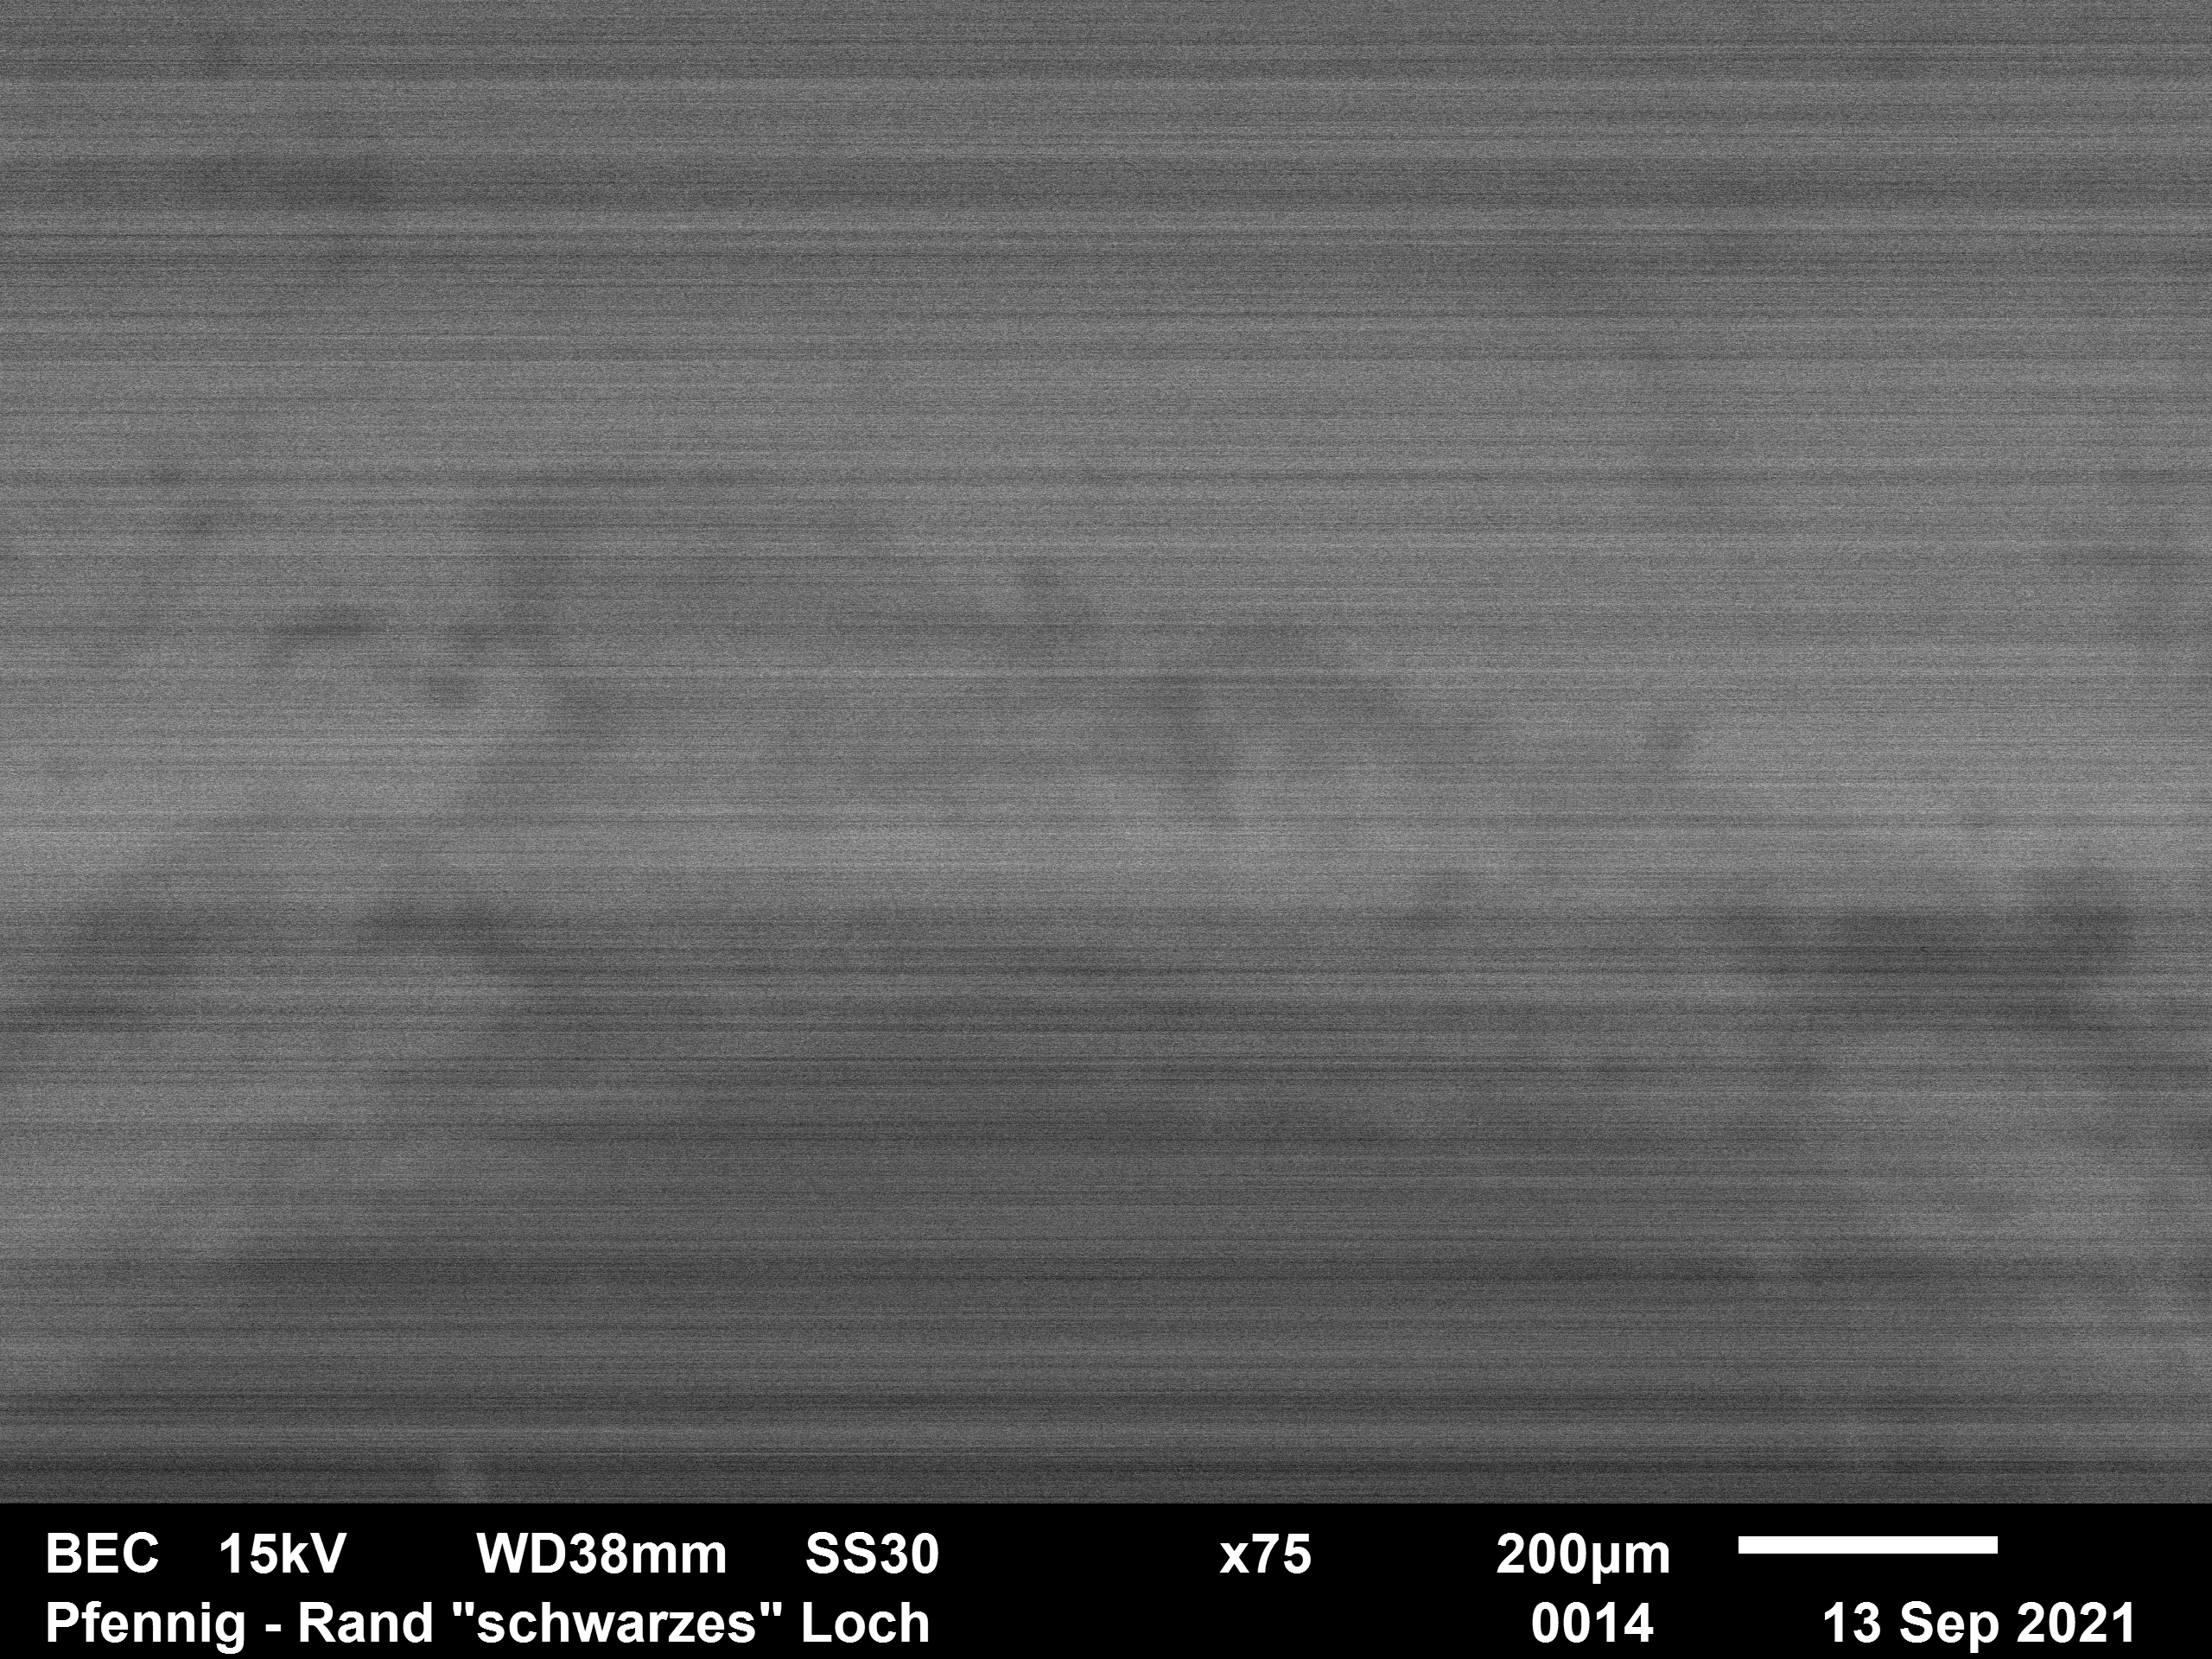
\includegraphics[width=\textwidth]{Auswertung/A/0014.png}
        \caption{$U_B = 15$ kV}
    \end{subfigure}
    \hfill
    \begin{subfigure}[b]{0.45\textwidth}
        \centering
        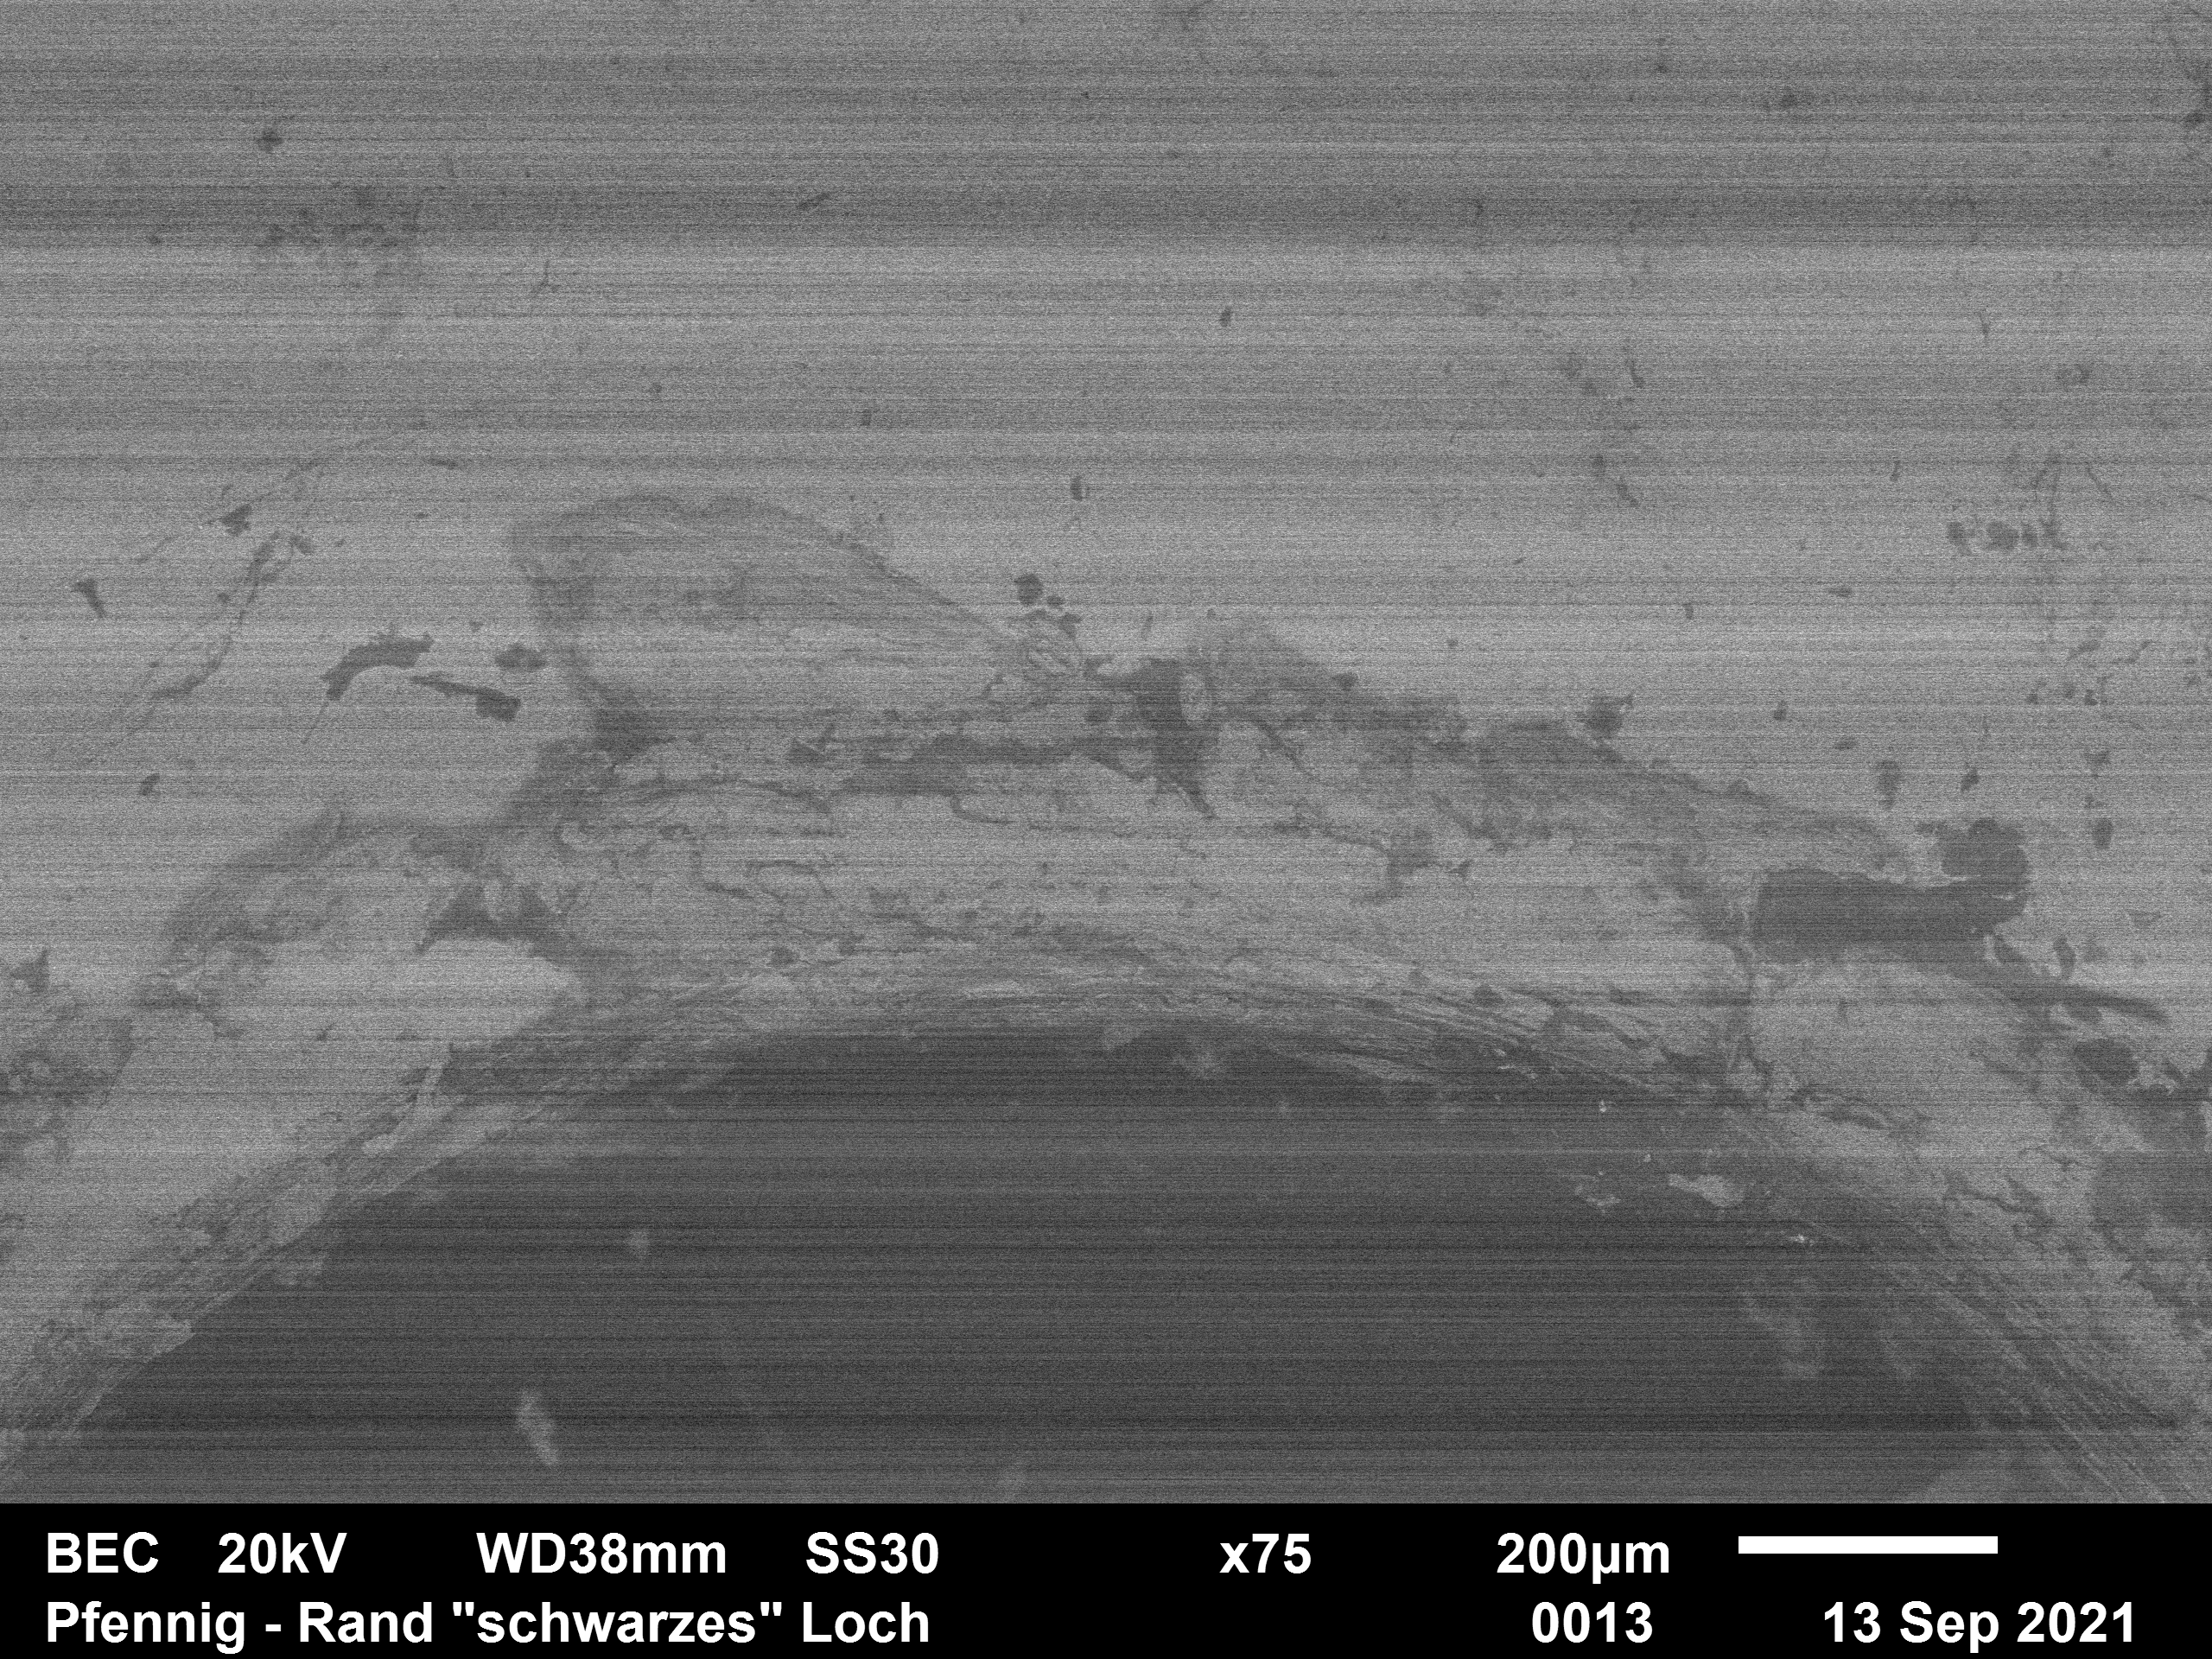
\includegraphics[width=\textwidth]{Auswertung/A/0013.png}
        \caption{$U_B = 20$ kV}
    \end{subfigure}
    \\
    \begin{subfigure}[b]{0.45\textwidth}
        \centering
        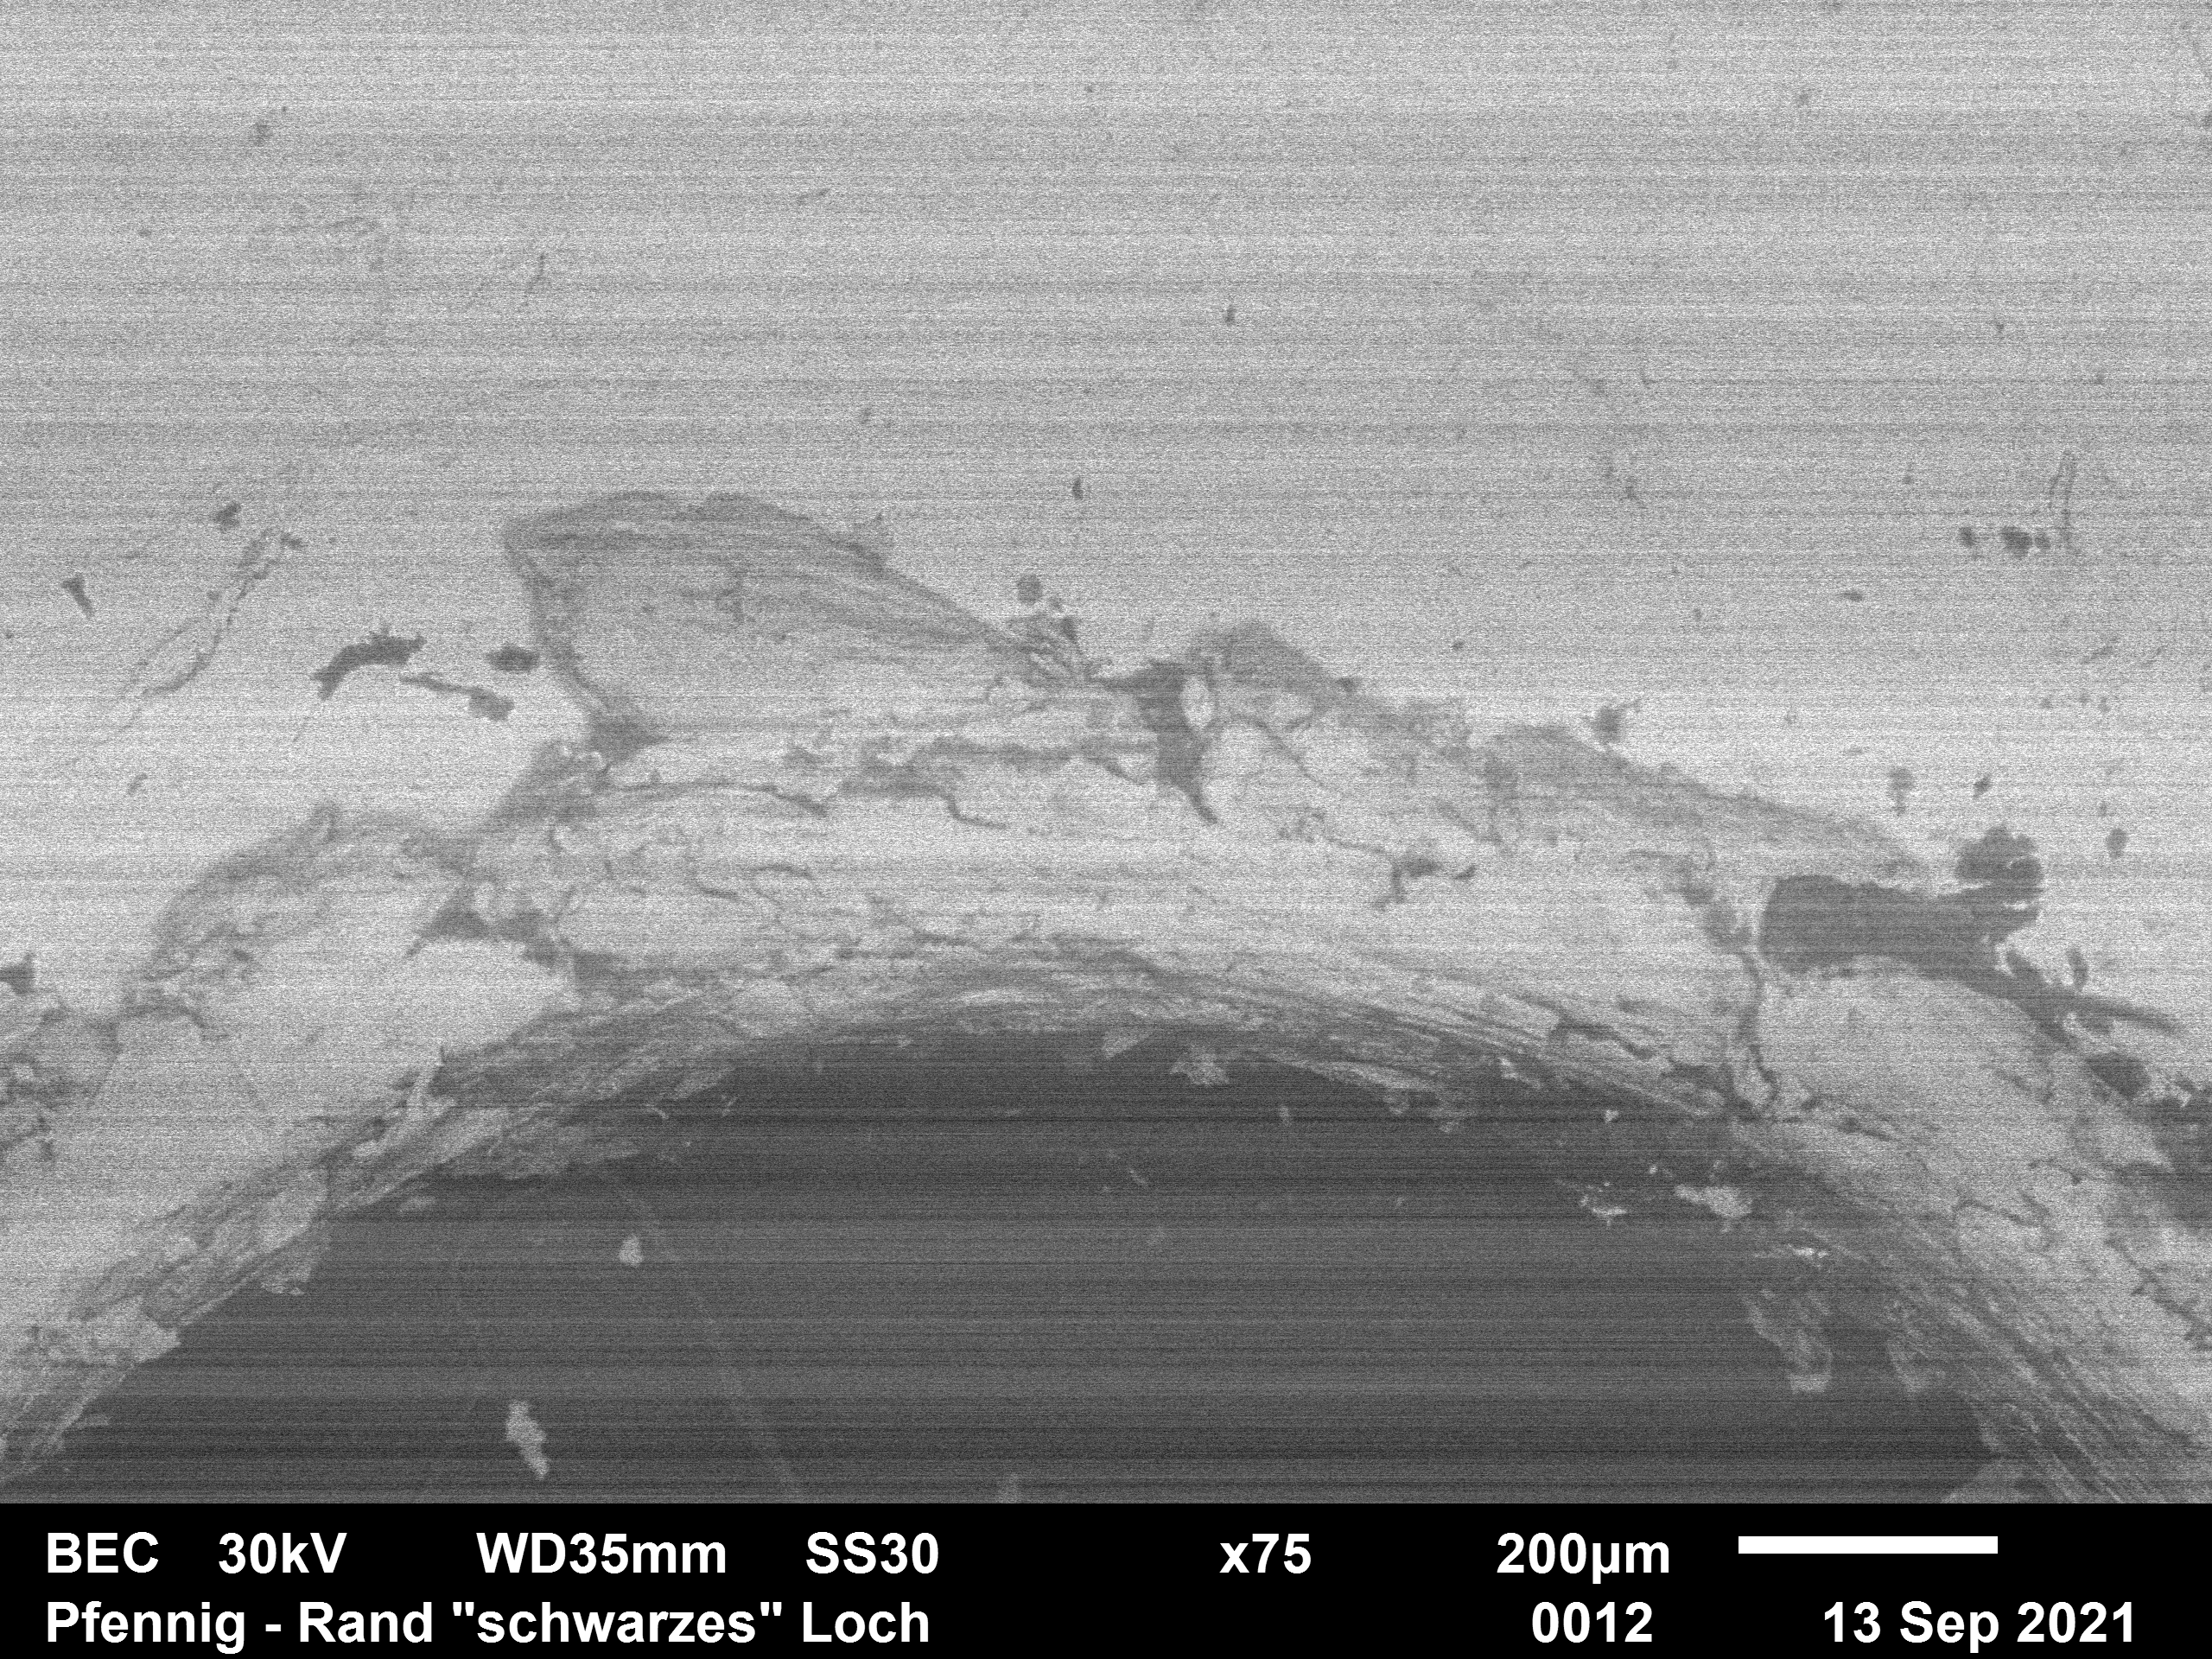
\includegraphics[width=\textwidth]{Auswertung/A/0012.png}
        \caption{$U_B = 30$ kV}
    \end{subfigure}
    \caption{BEC bei unterschiedlichen Beschleunigunsspannungen}
\end{figure}

Diskussion!

\newpage
Auch für den Halbleiterdetektor im Topo-Mode (BET) wurde die Beschleunigungsspannung variiert.
\begin{figure}[h]
    \centering
    
    \begin{subfigure}[b]{0.45\textwidth}
        \centering
        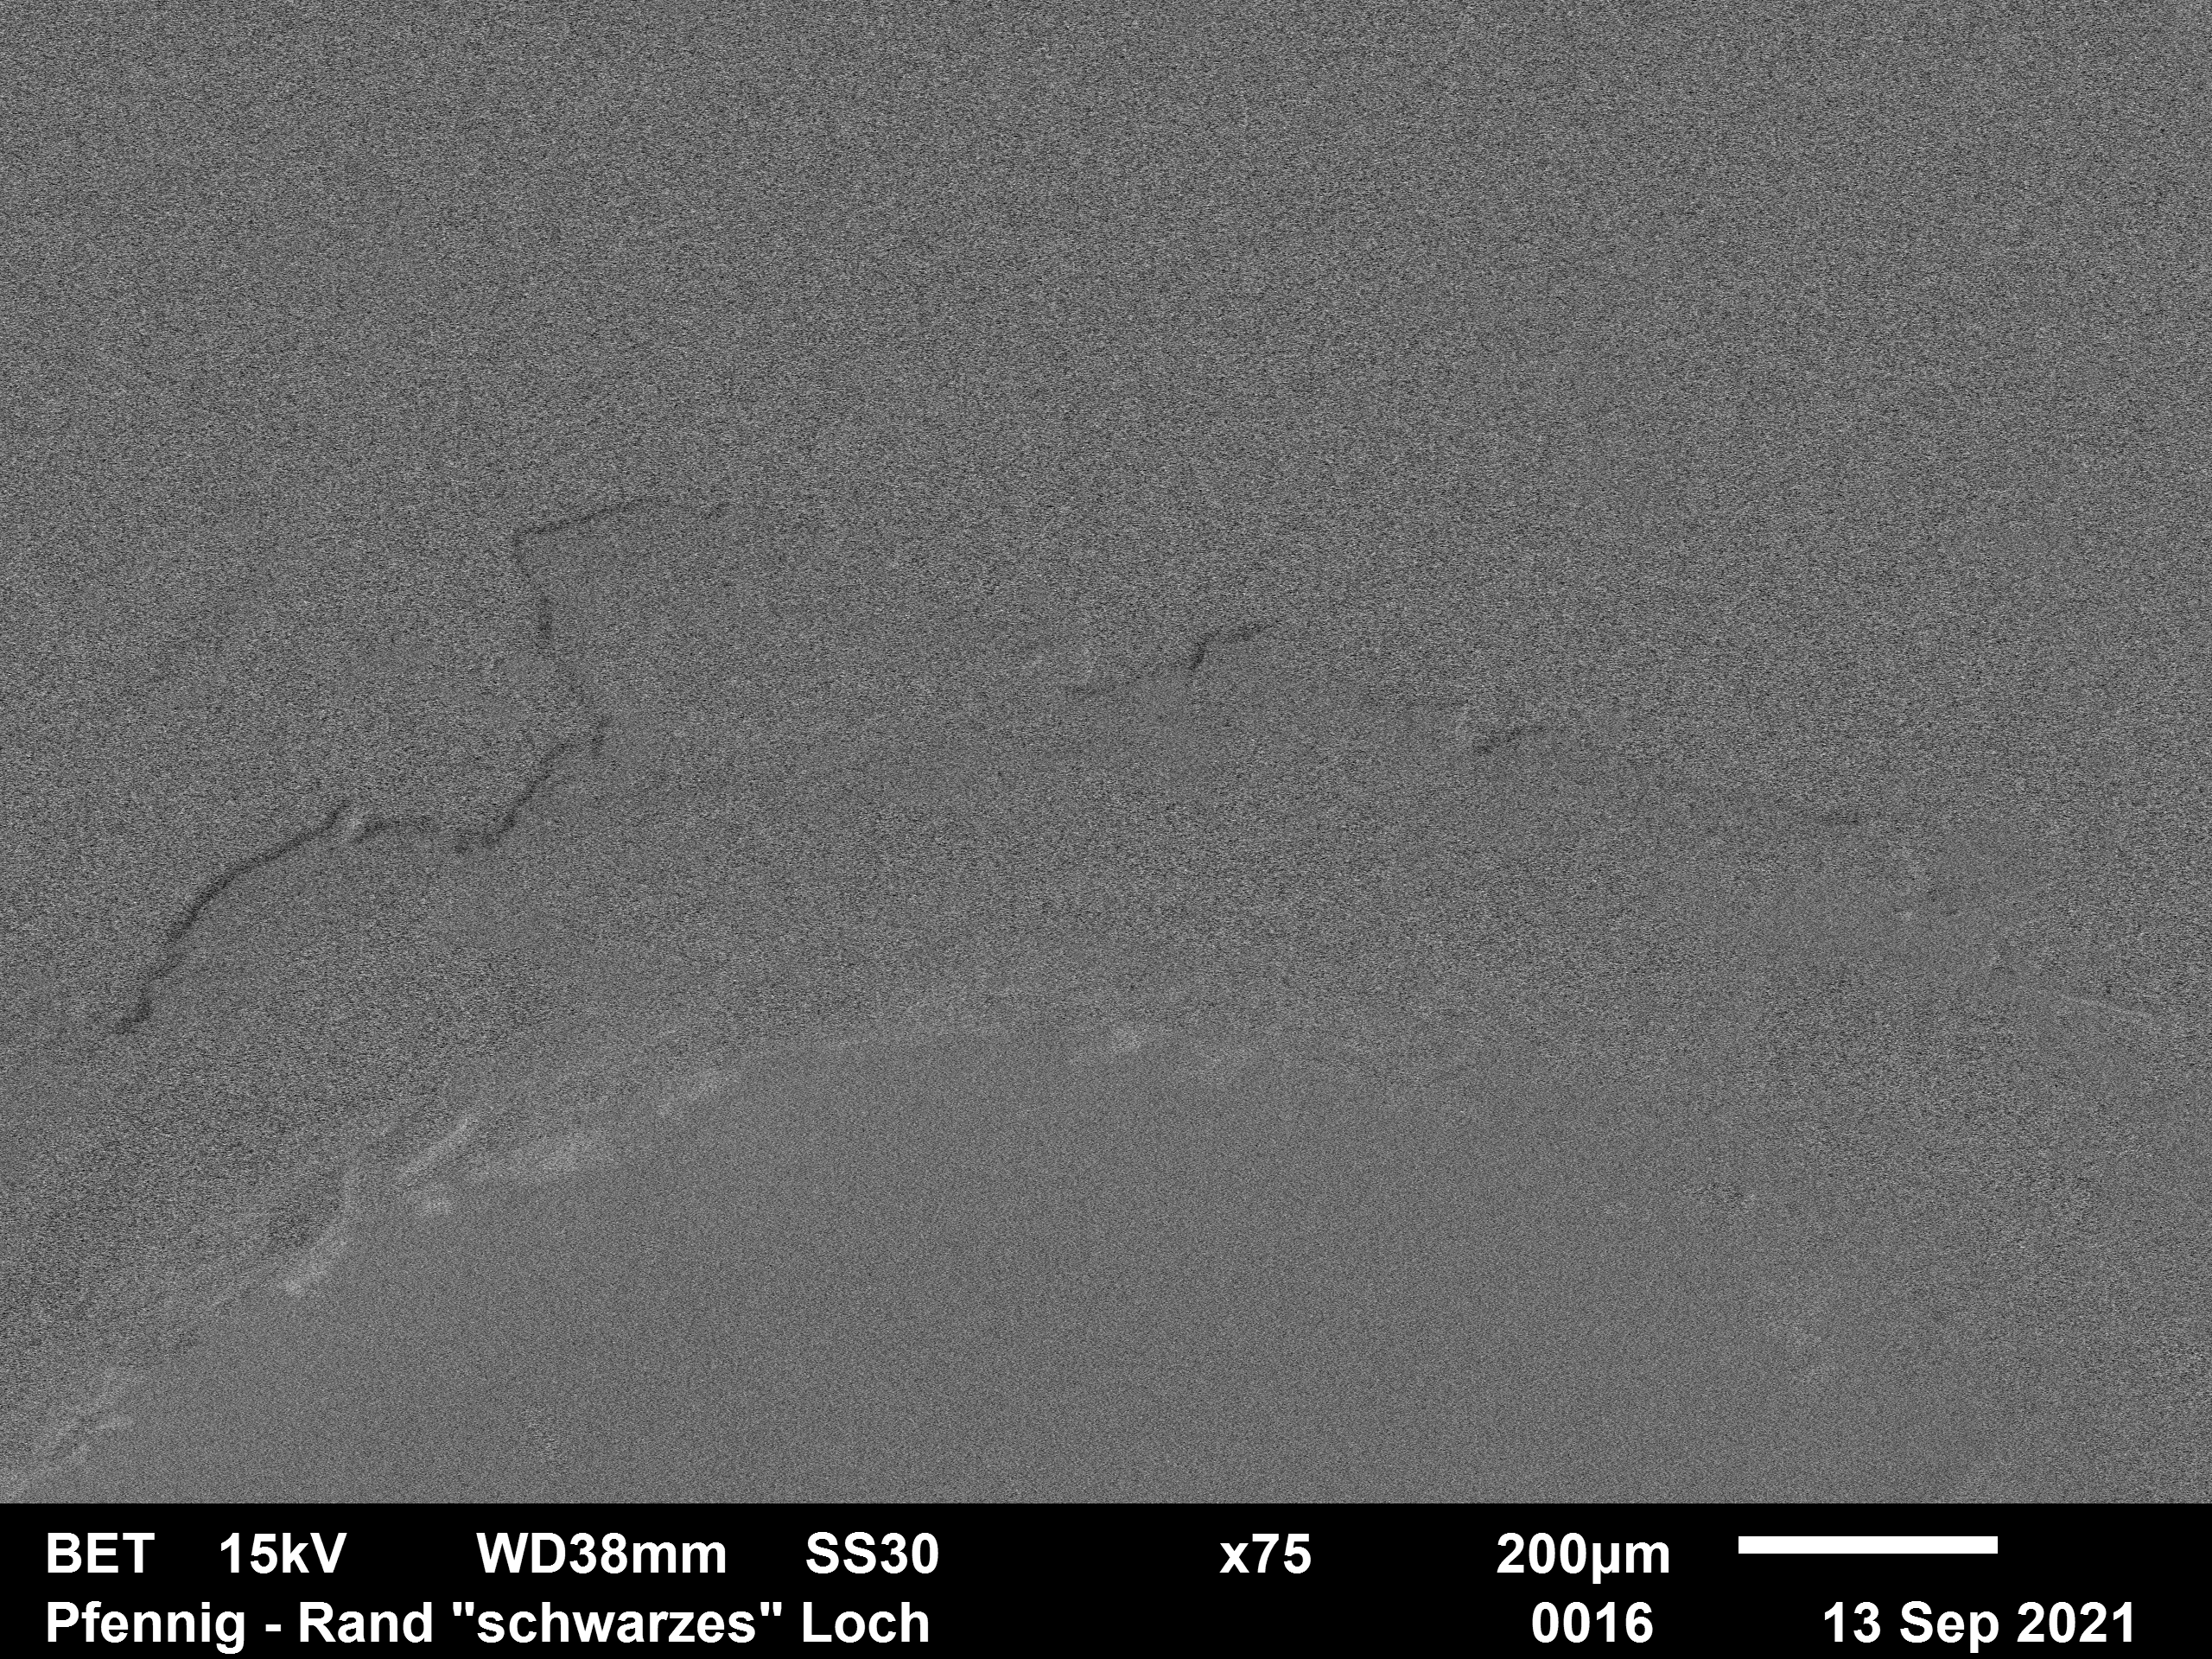
\includegraphics[width=\textwidth]{Auswertung/A/0016.png}
        \caption{$U_B = 15$ kV}
    \end{subfigure}
    \hfill
    \begin{subfigure}[b]{0.45\textwidth}
        \centering
        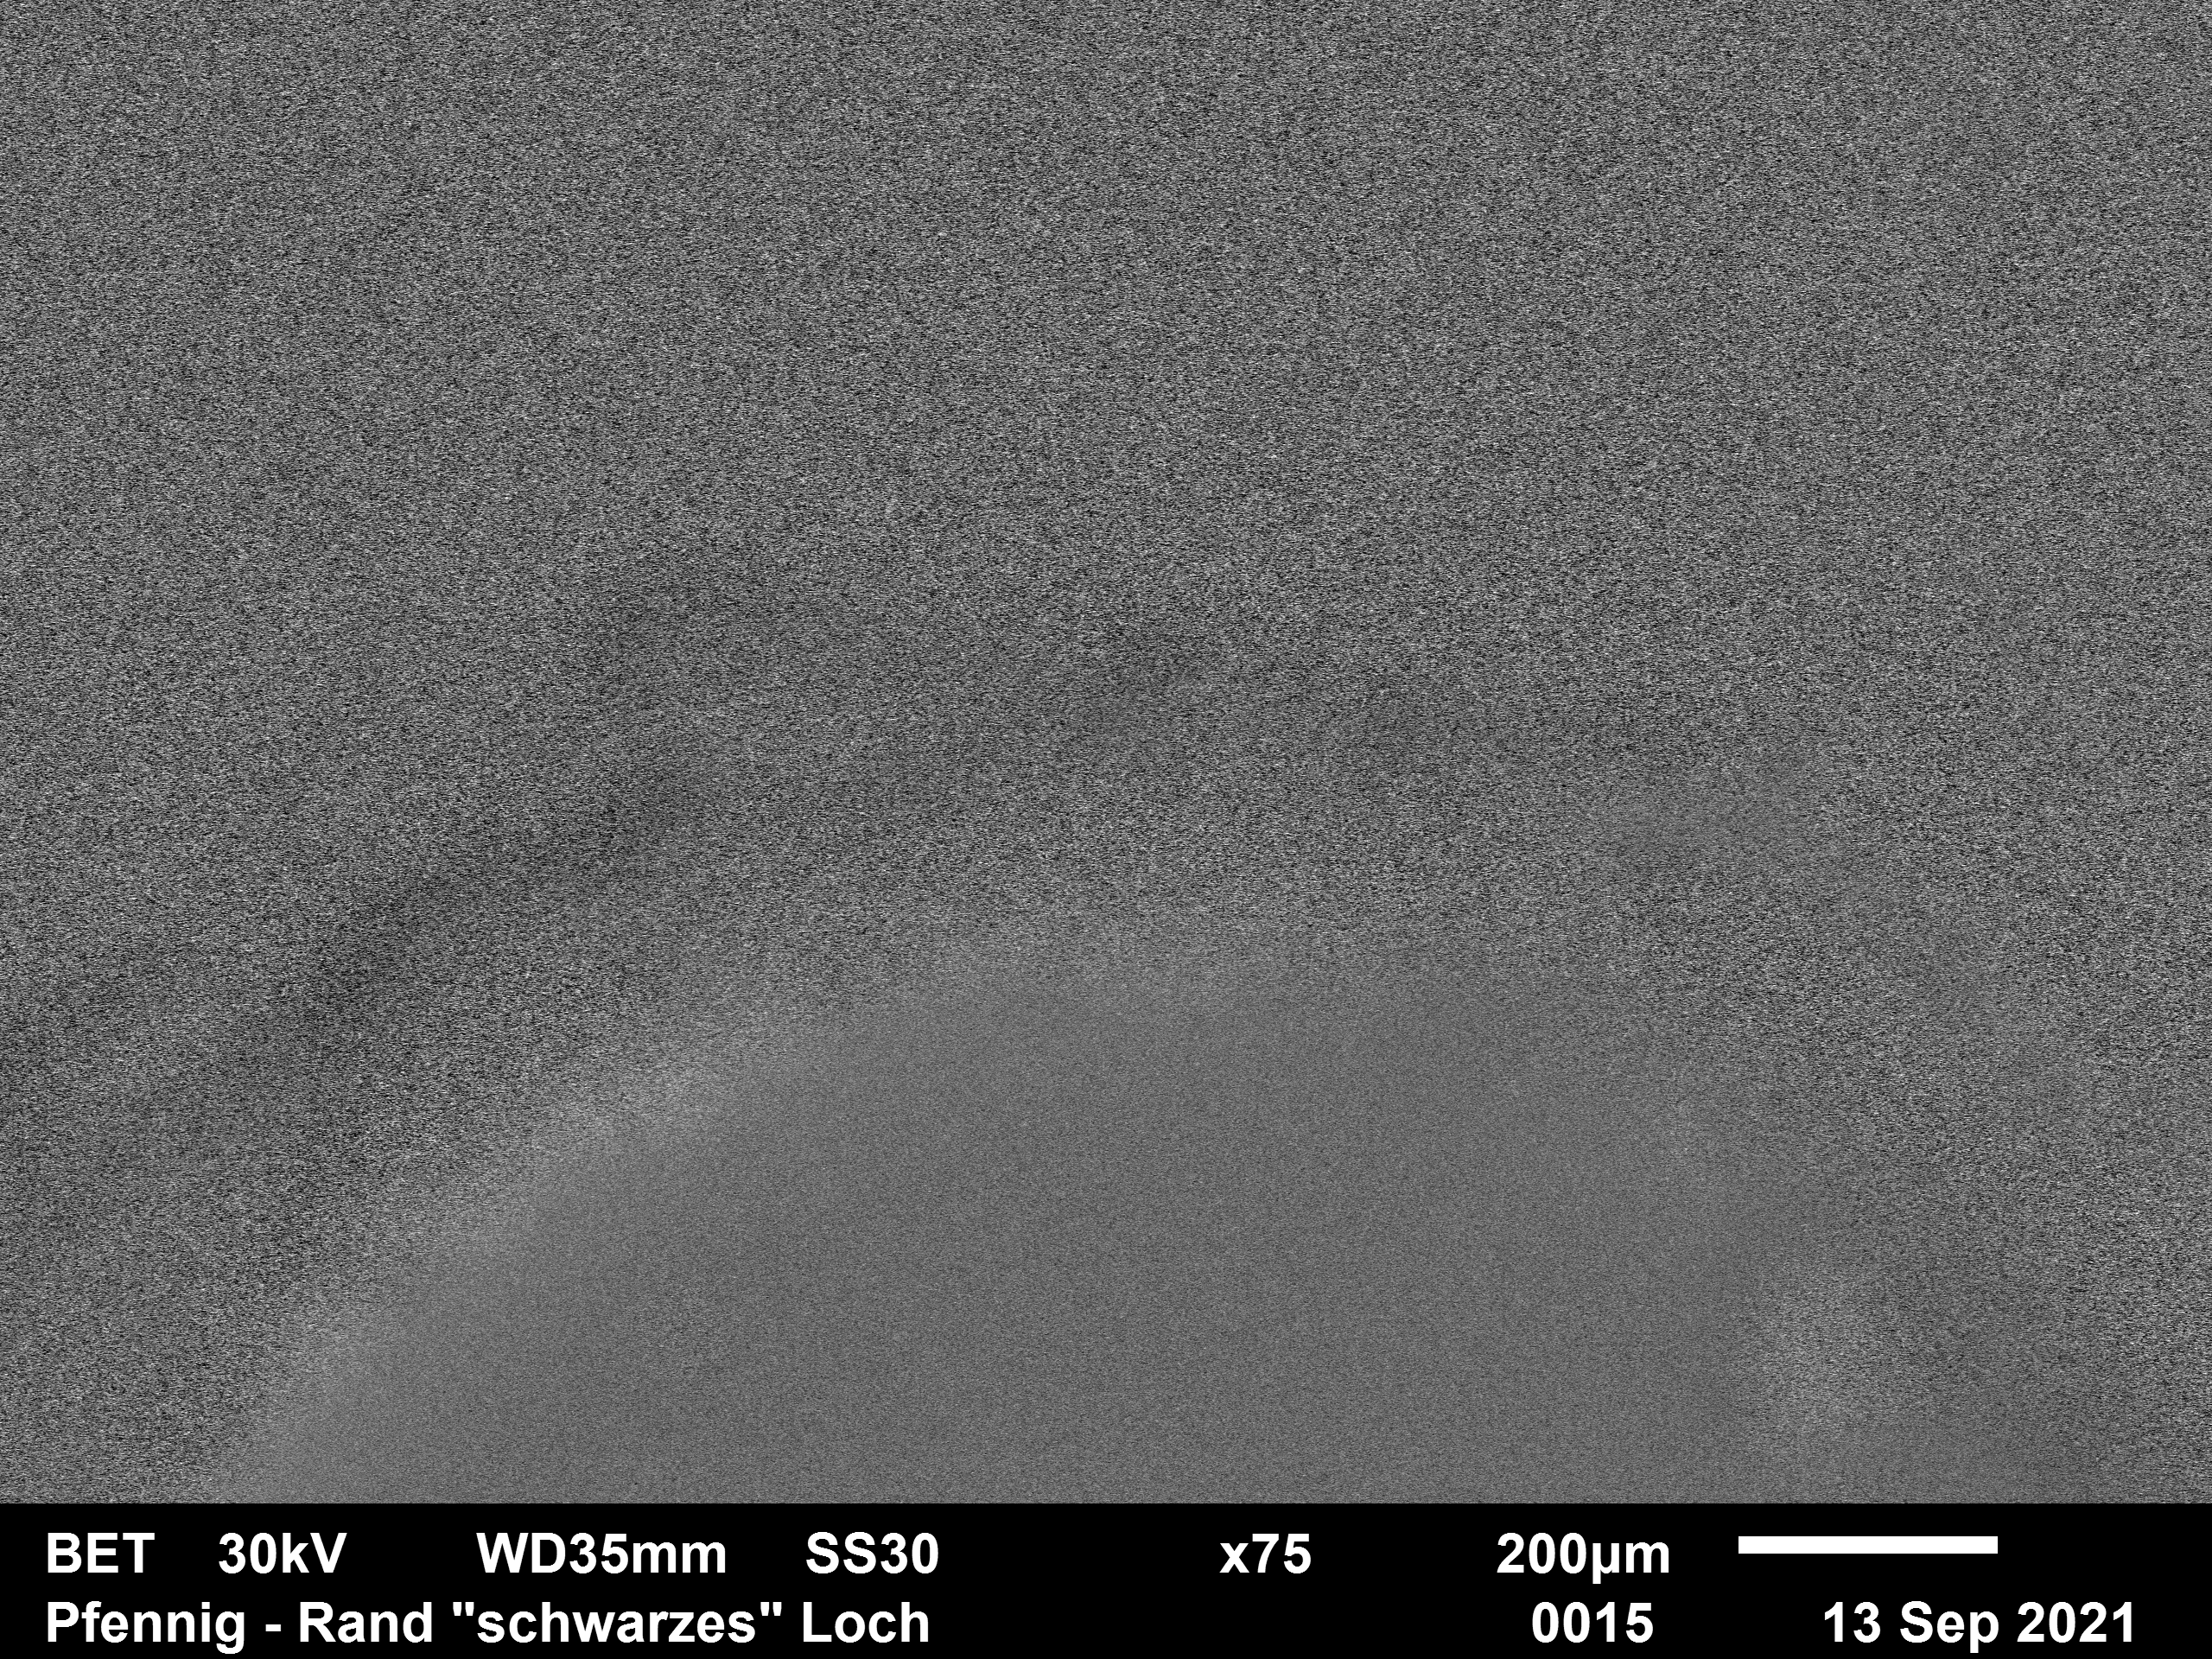
\includegraphics[width=\textwidth]{Auswertung/A/0015.png}
        \caption{$U_B = 30$ kV}
    \end{subfigure}
    
    \caption{BET bei unterschiedlichen Beschleunigunsspannungen}
\end{figure}

Diskussion!

\newpage
Außerdem wurde eine Stelle mit verschiedenen Strahldurschmessern abgetastet.
\begin{figure}[h]
    \centering
    
    \begin{subfigure}[b]{0.45\textwidth}
        \centering
        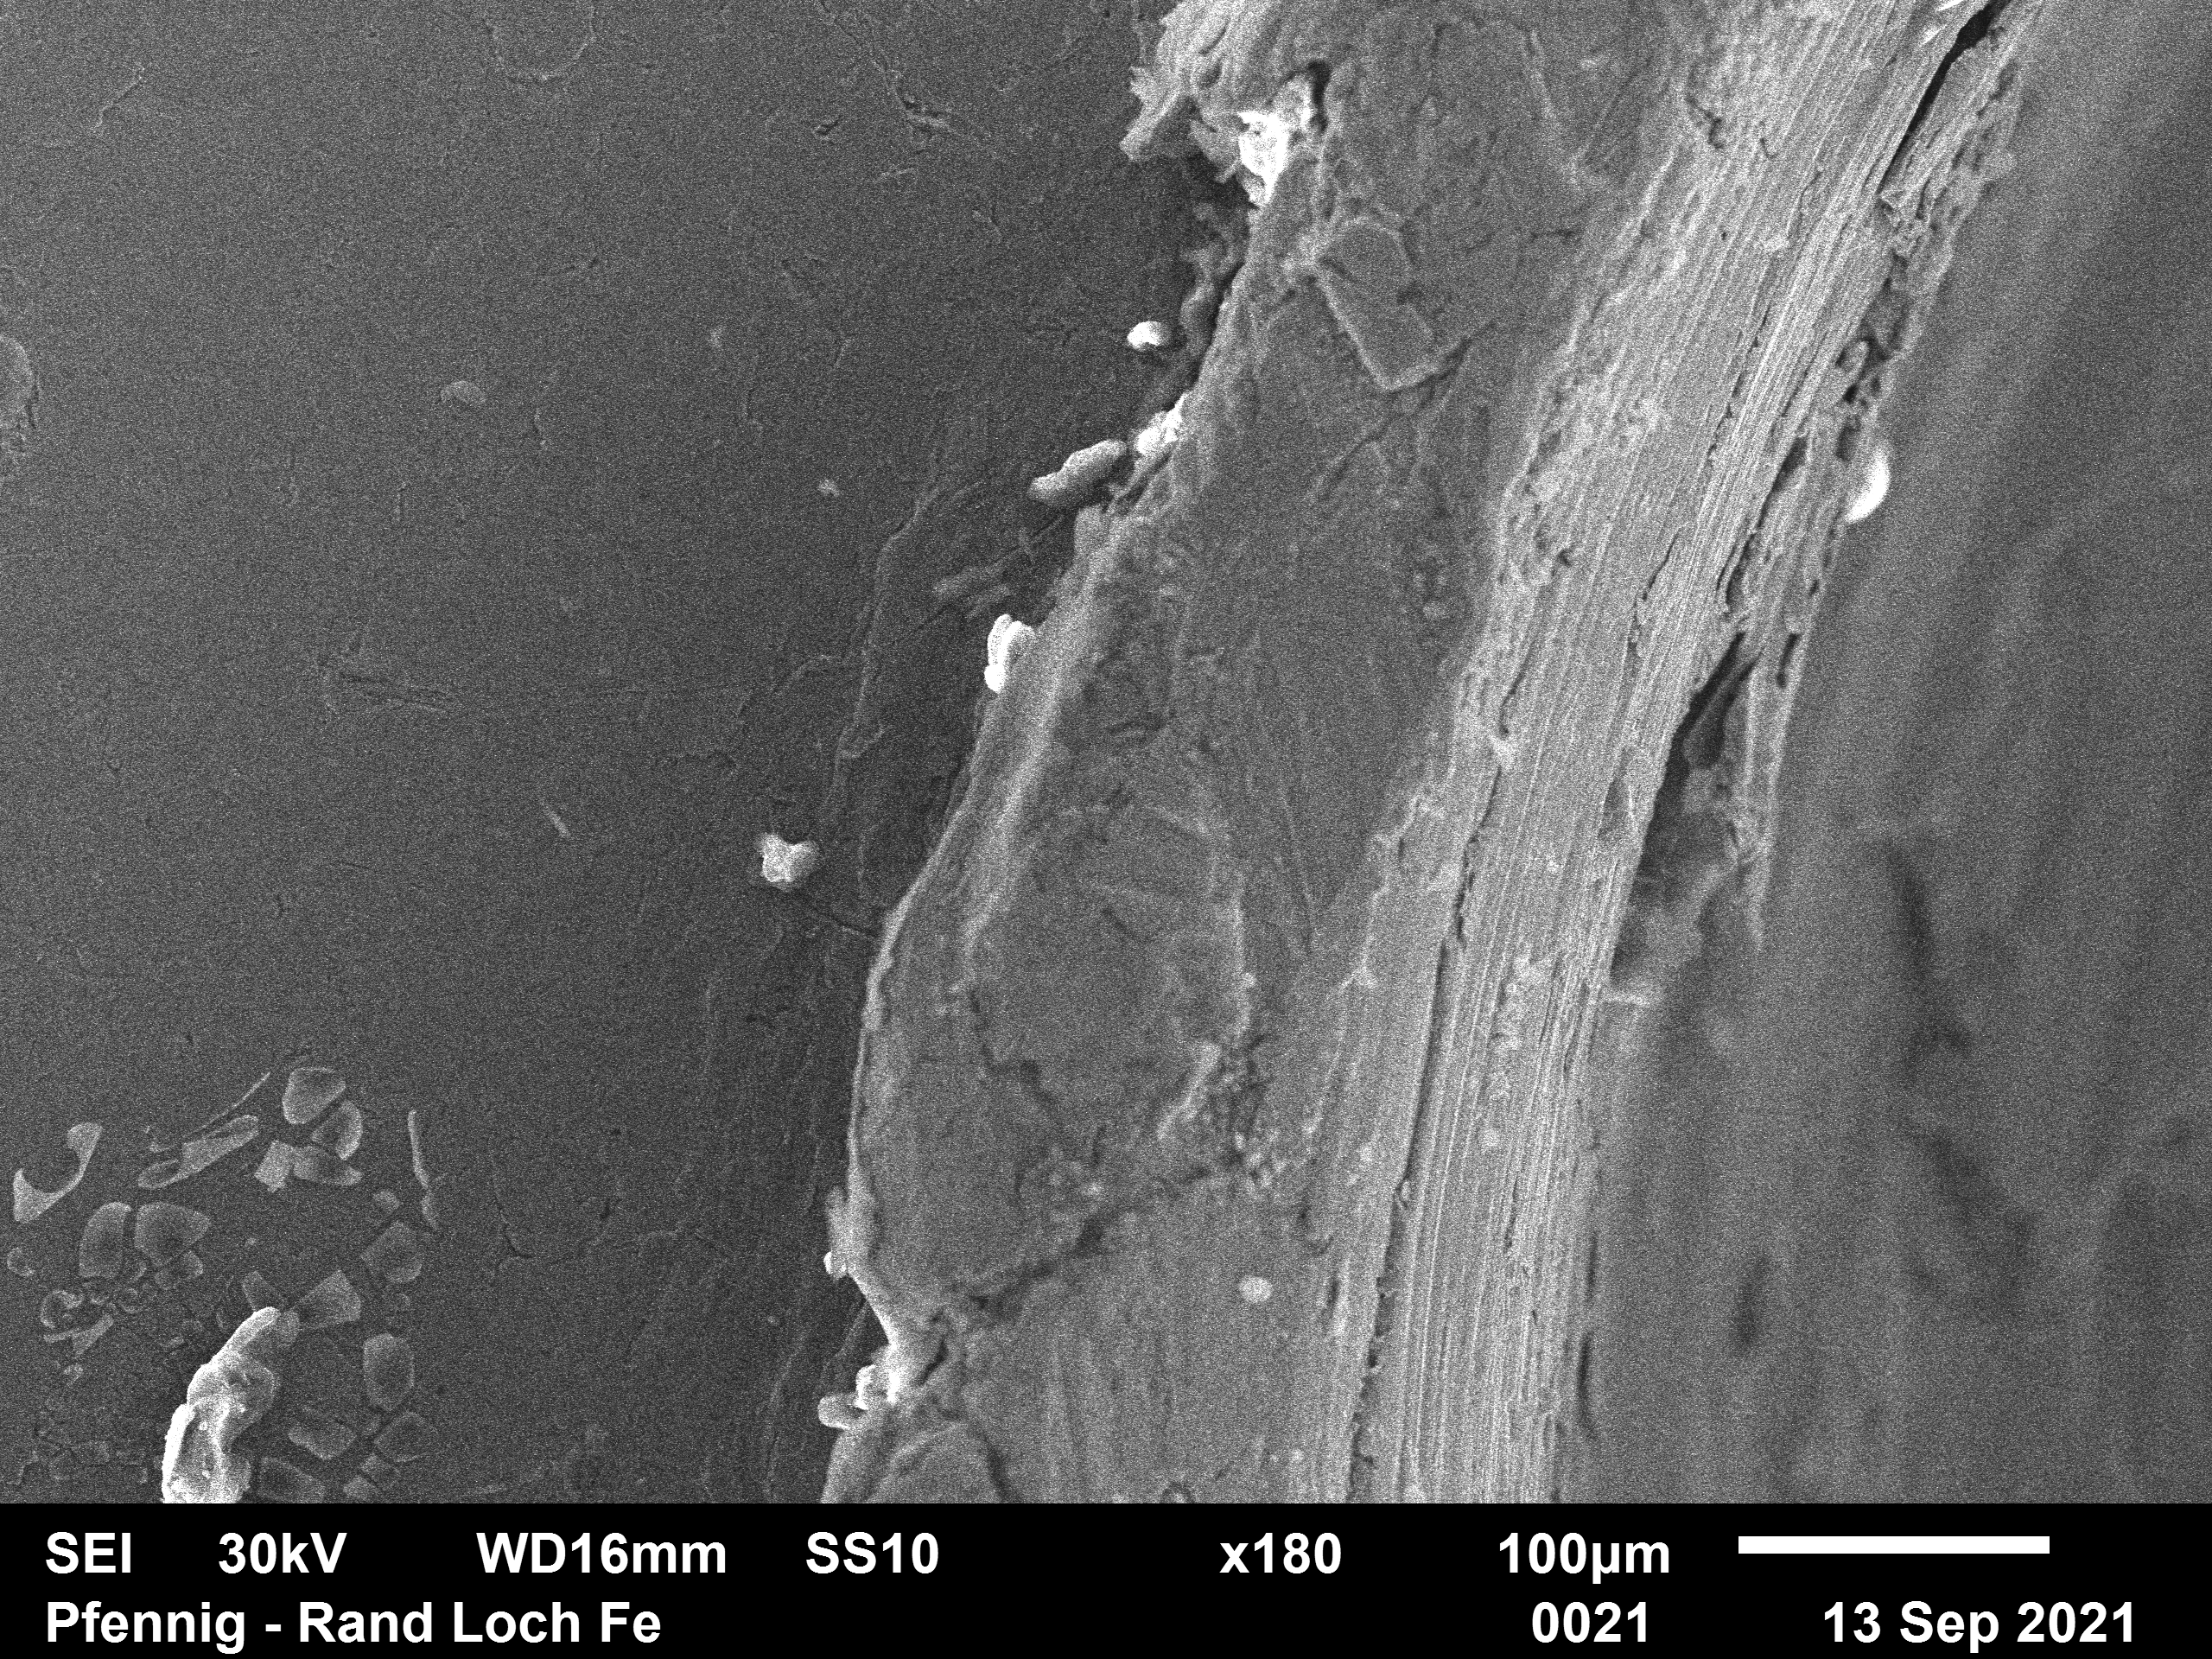
\includegraphics[width=\textwidth]{Auswertung/A/0021.png}
        \caption{SS 10}
    \end{subfigure}
    \hfill
    \begin{subfigure}[b]{0.45\textwidth}
        \centering
        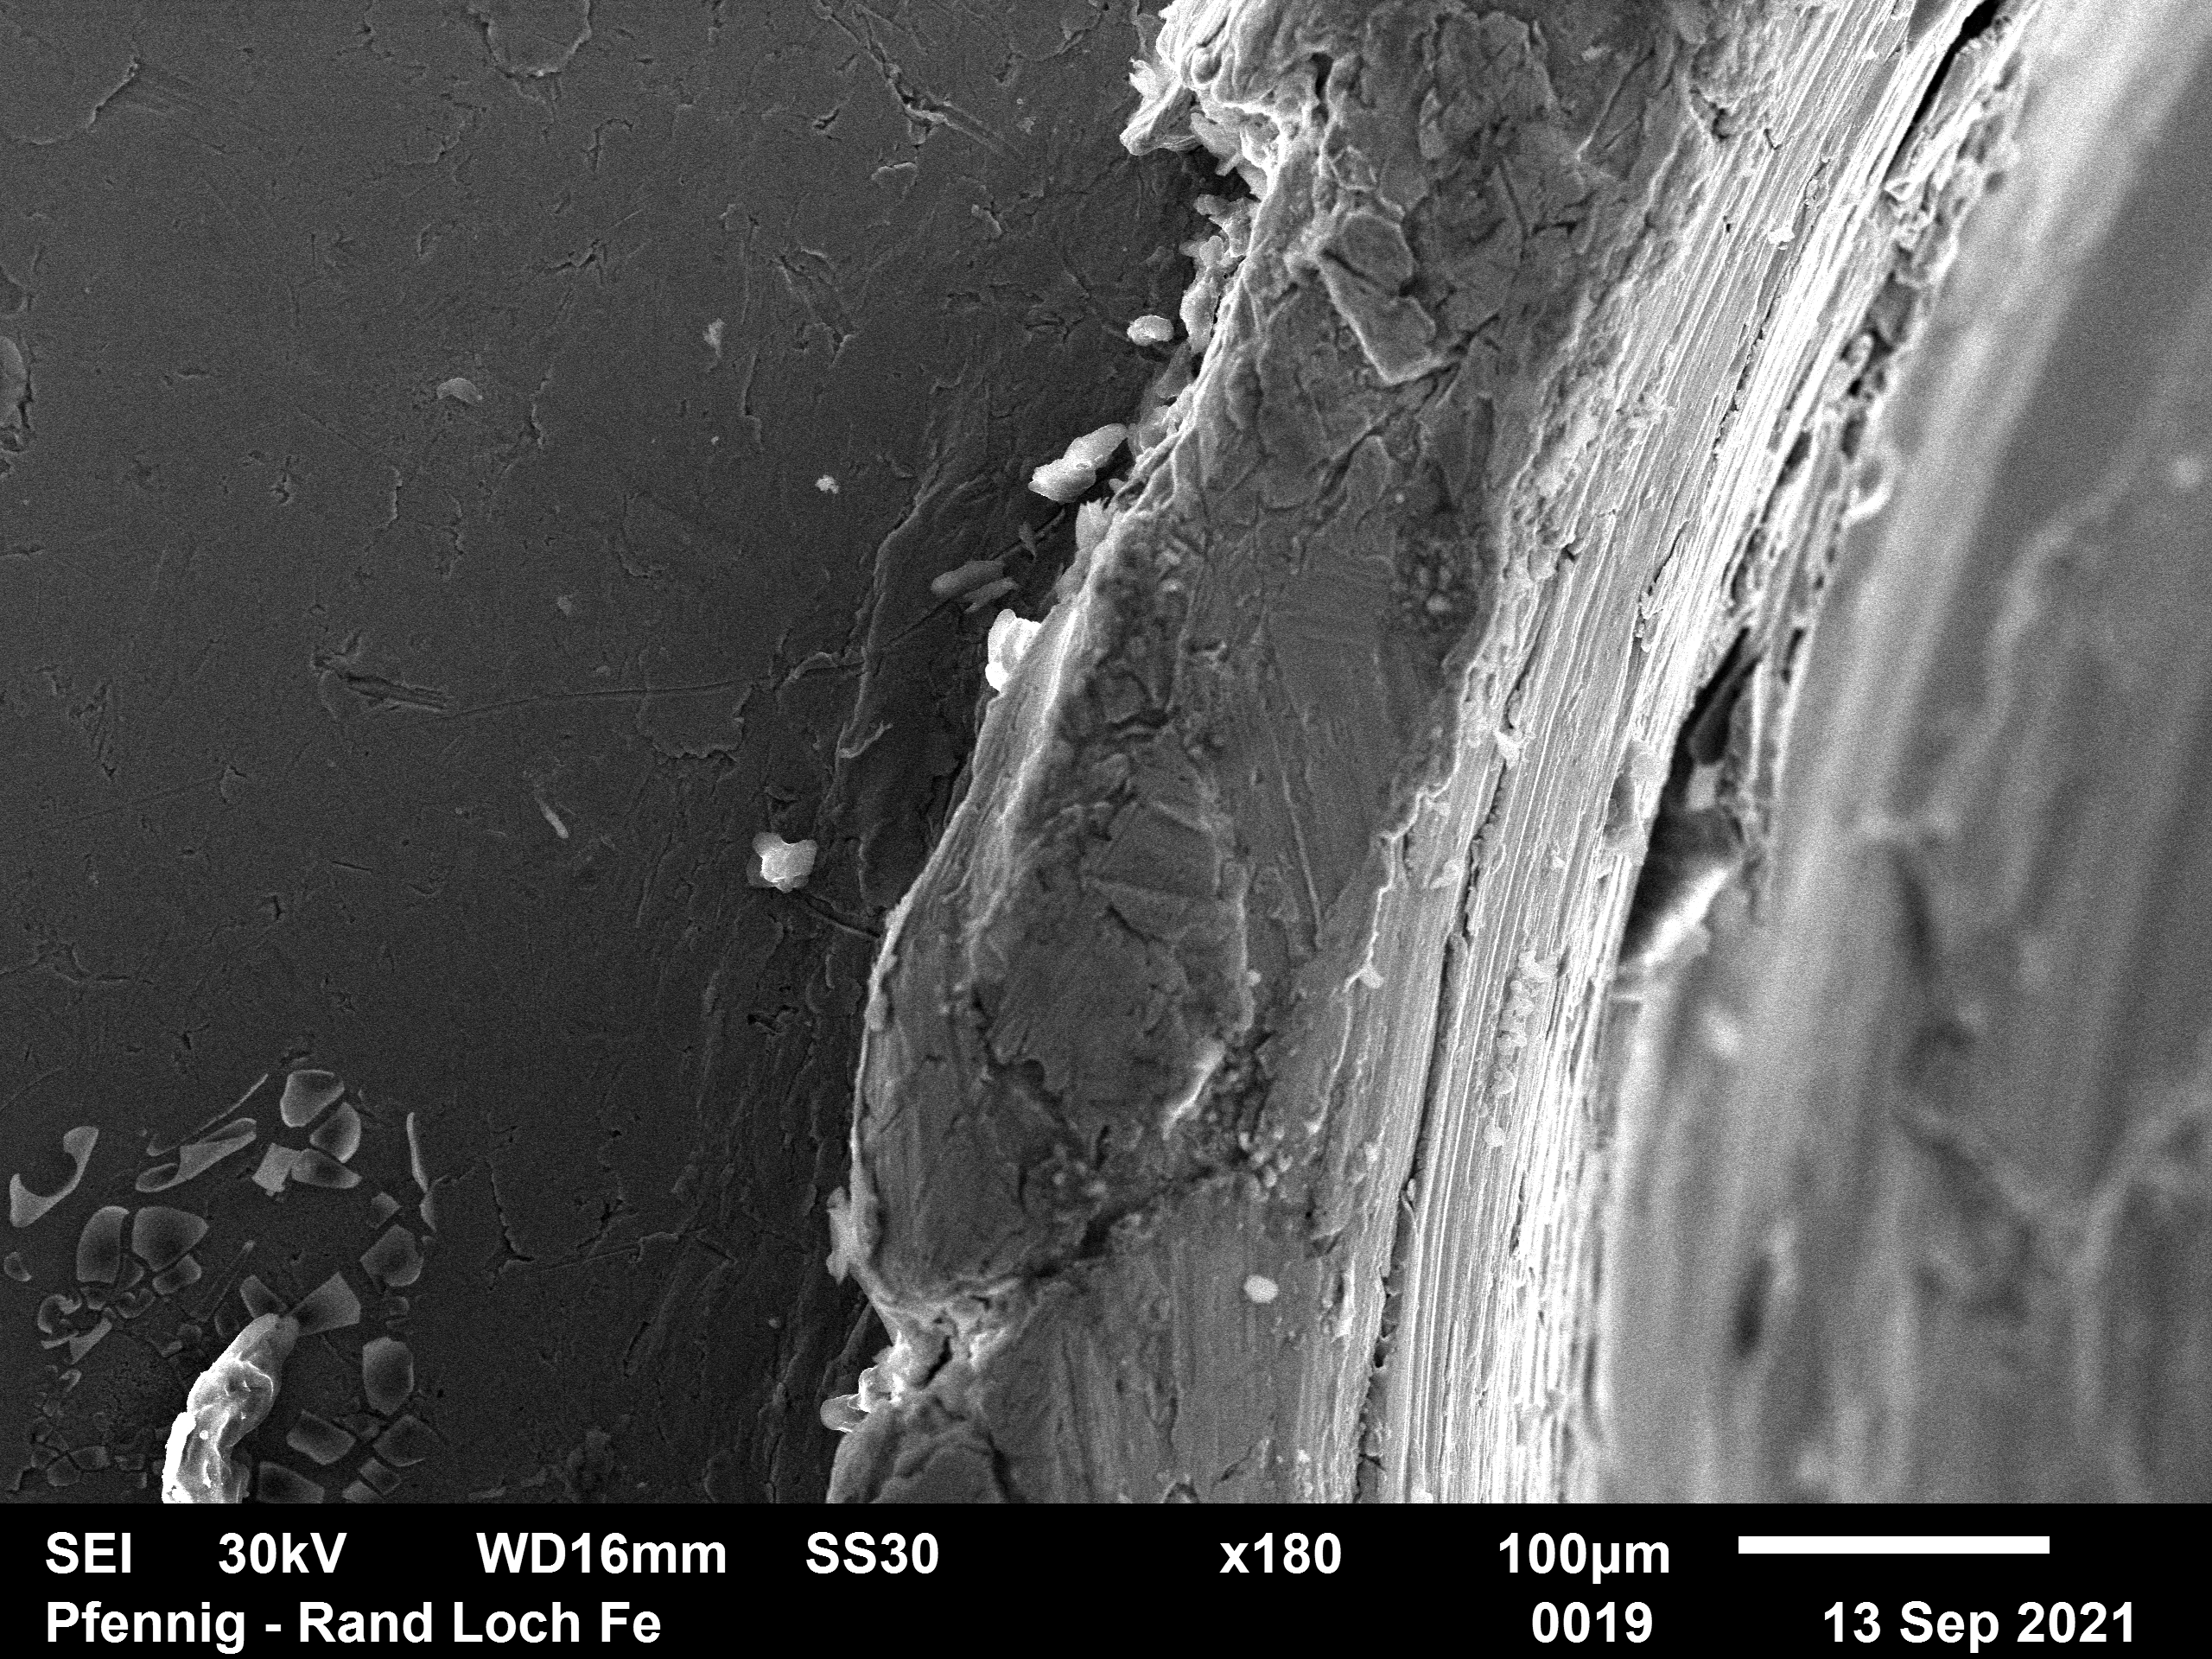
\includegraphics[width=\textwidth]{Auswertung/A/0019.png}
        \caption{SS 30}
    \end{subfigure}
    \\
    \begin{subfigure}[b]{0.45\textwidth}
        \centering
        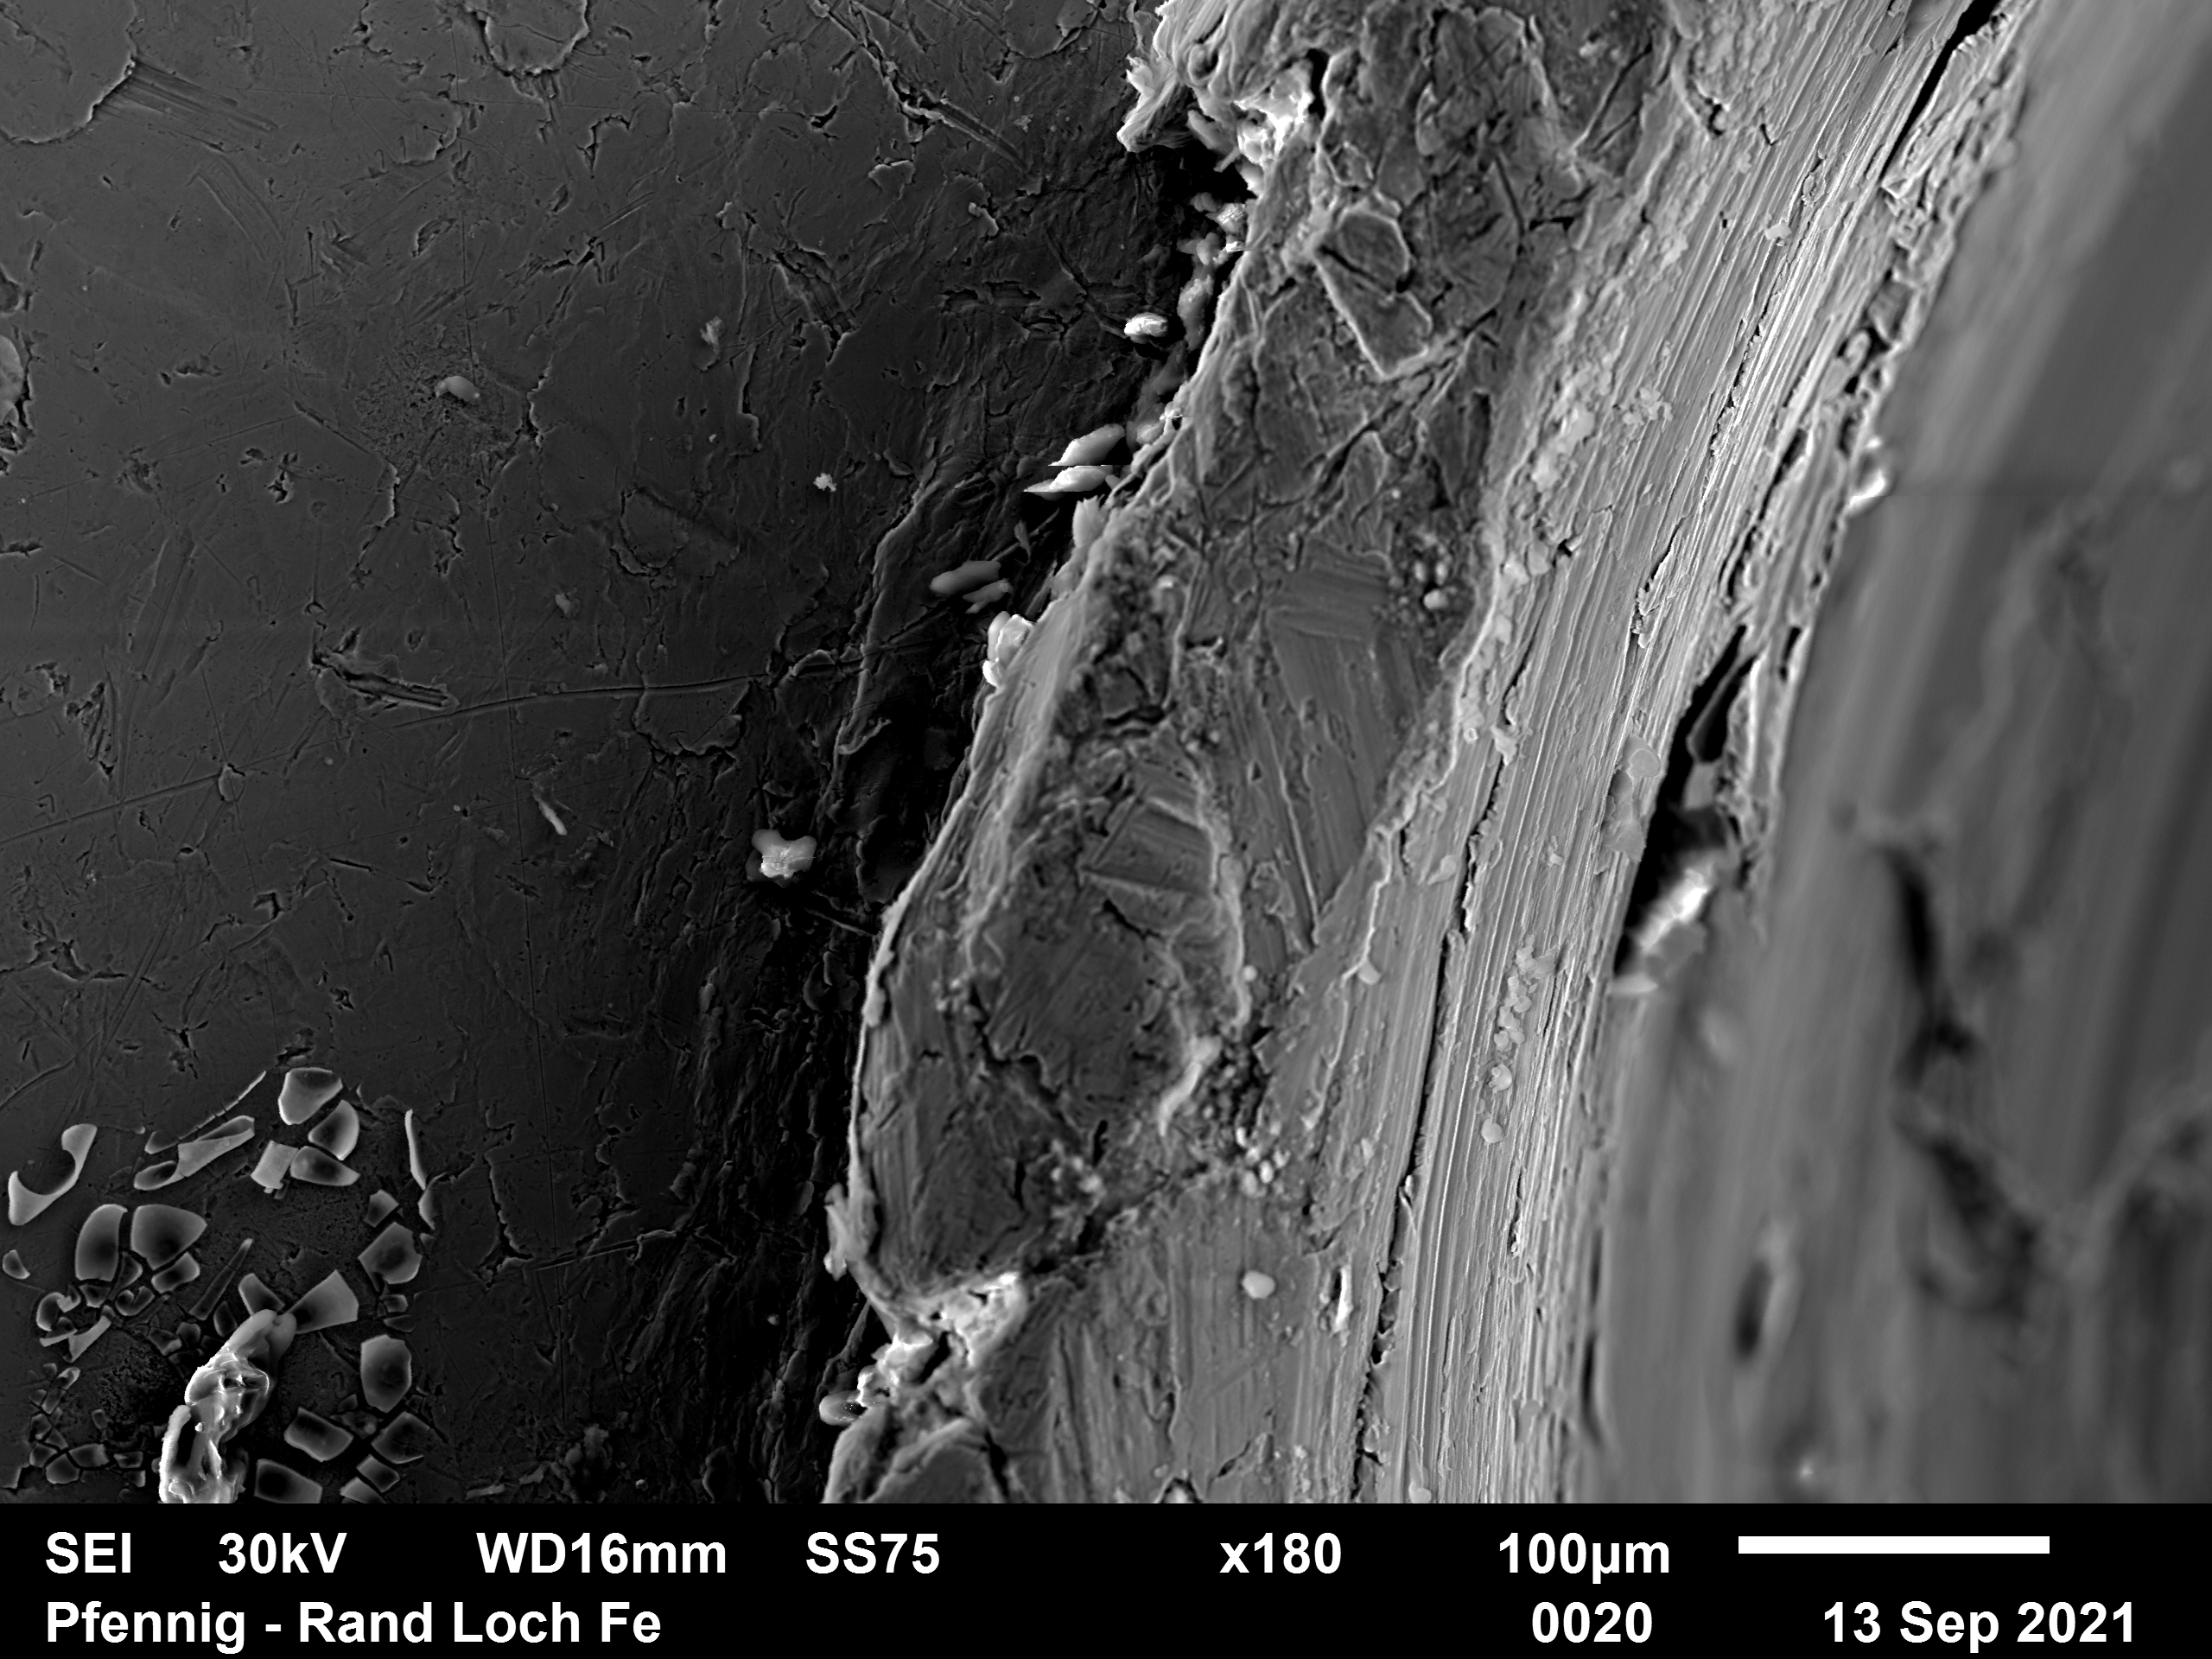
\includegraphics[width=\textwidth]{Auswertung/A/0020.png}
        \caption{SS 75}
    \end{subfigure}
    \caption{SEI bei unterschiedlichen Strahldurschmessern}
\end{figure}

Diskussion !

\newpage
\subsection{EDX Analyse}
Nun sollen das Röntgenspektrum der Münze, sowie des gefüllten Lochs mithilfe des EDX Detektors aufgezeichnet werden. Mit dessen Hilfe kann die Materialzusammensetzung ermittelt werden. \\

Zuerst wurde das Spektrum der Münze aufgenommen: 
\begin{figure}[h]
    \centering
    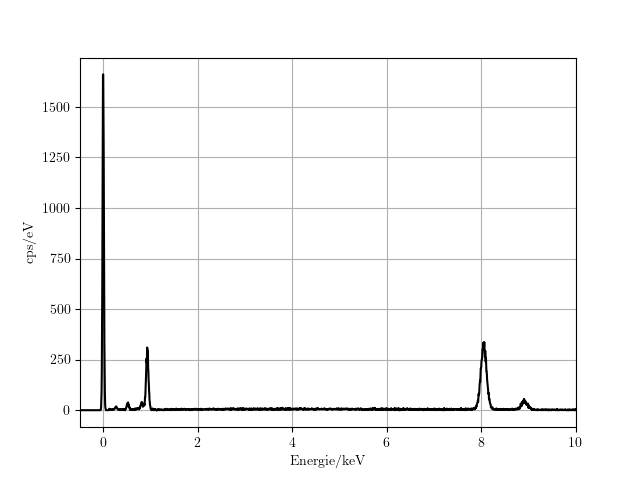
\includegraphics[width=\textwidth]{Auswertung/A/EdxFl.png}
    \caption{Röntgenspektrum der Kupfermünze}
\end{figure}

Markierung der Peaks!\\
Diskussion!\\

\begin{table}[h]
    \centering
    \begin{tabular}{c|c|c|c|c|c|c}
        Element & OZ &Serie& unn. C & norm. C &  Atom. C  & Fehler (1 Sigma) \\
         & & & [Gew. \%] & [Gew. \%] & [At. \%] & [Gew. \%] \\
        \hline\hline
        C & 6 & K & 13,96&11,87&23,84 & 35,27\\
        O & 8 & K & 10,72&9,11&20,33 & 3,41\\
        Cu & 29 & K & 92,94&79,02&44,40 & 2,50\\
    \end{tabular}
    \caption{Ergebnisse der EDX-Analyse der Kupfermünze}
\end{table}

\newpage
Anschließend wurde das Spektrum des Materials in einem der Löcher aufgenommen: 
\begin{figure}[h]
    \centering
    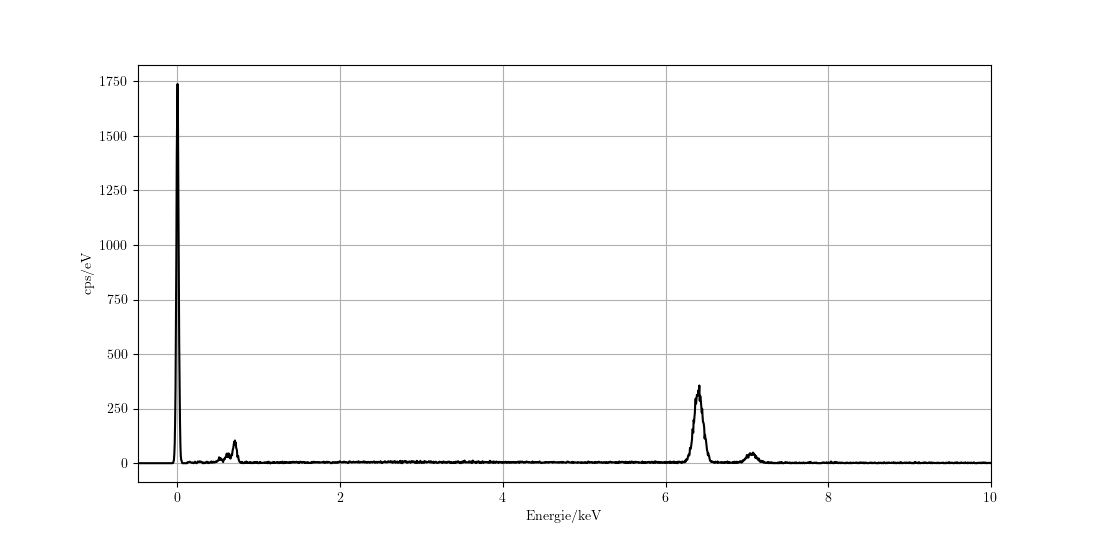
\includegraphics[width=\textwidth]{Auswertung/A/EdxLoch.png}
    \caption{Röntgenspektrum des Fremdmaterials}
\end{figure}

Markierung der Peaks!\\
Diskussion!\\

\begin{table}[h]
    \centering
    \begin{tabular}{c|c|c|c|c|c|c}
        Element & OZ &Serie& unn. C & norm. C &  Atom. C  & Fehler (1 Sigma) \\
         & & & [Gew. \%] & [Gew. \%] & [At. \%] & [Gew. \%] \\
        \hline\hline
        C & 6 & K & 7,06&7,57&23,84 & 4,17\\
        O & 8 & K & 7,52&8,06&19,05 & 2,83\\
        Fe & 26 & K & 78,68&84,36&57,11 & 2,19\\
    \end{tabular}
    \caption{Ergebnisse der EDX-Analyse des Fremdmaterials}
\end{table}

\newpage
\section{Fliege}

Als nächste Probe wurde eine Fliege eingelegt. Da es sich hierbei um organisches Material handelt wurde sie mit Gold bedampft, um eine Untersuchung möglich zu machen. Weiterhin ist darauf zu achten, die Beschleunigungsspannung nicht zu groß (ca. 10  kV) einzustellen, da die Probe sonst beschädigt werden kann. \\

Zuerst wurde die Flieg im Ganzen aufgenommen. Um dabei eine höhe Tiefenschärfe zu erreichen wurde ein großer Arbeitsabstand eingestellt.
\begin{figure}[h]
    \centering
    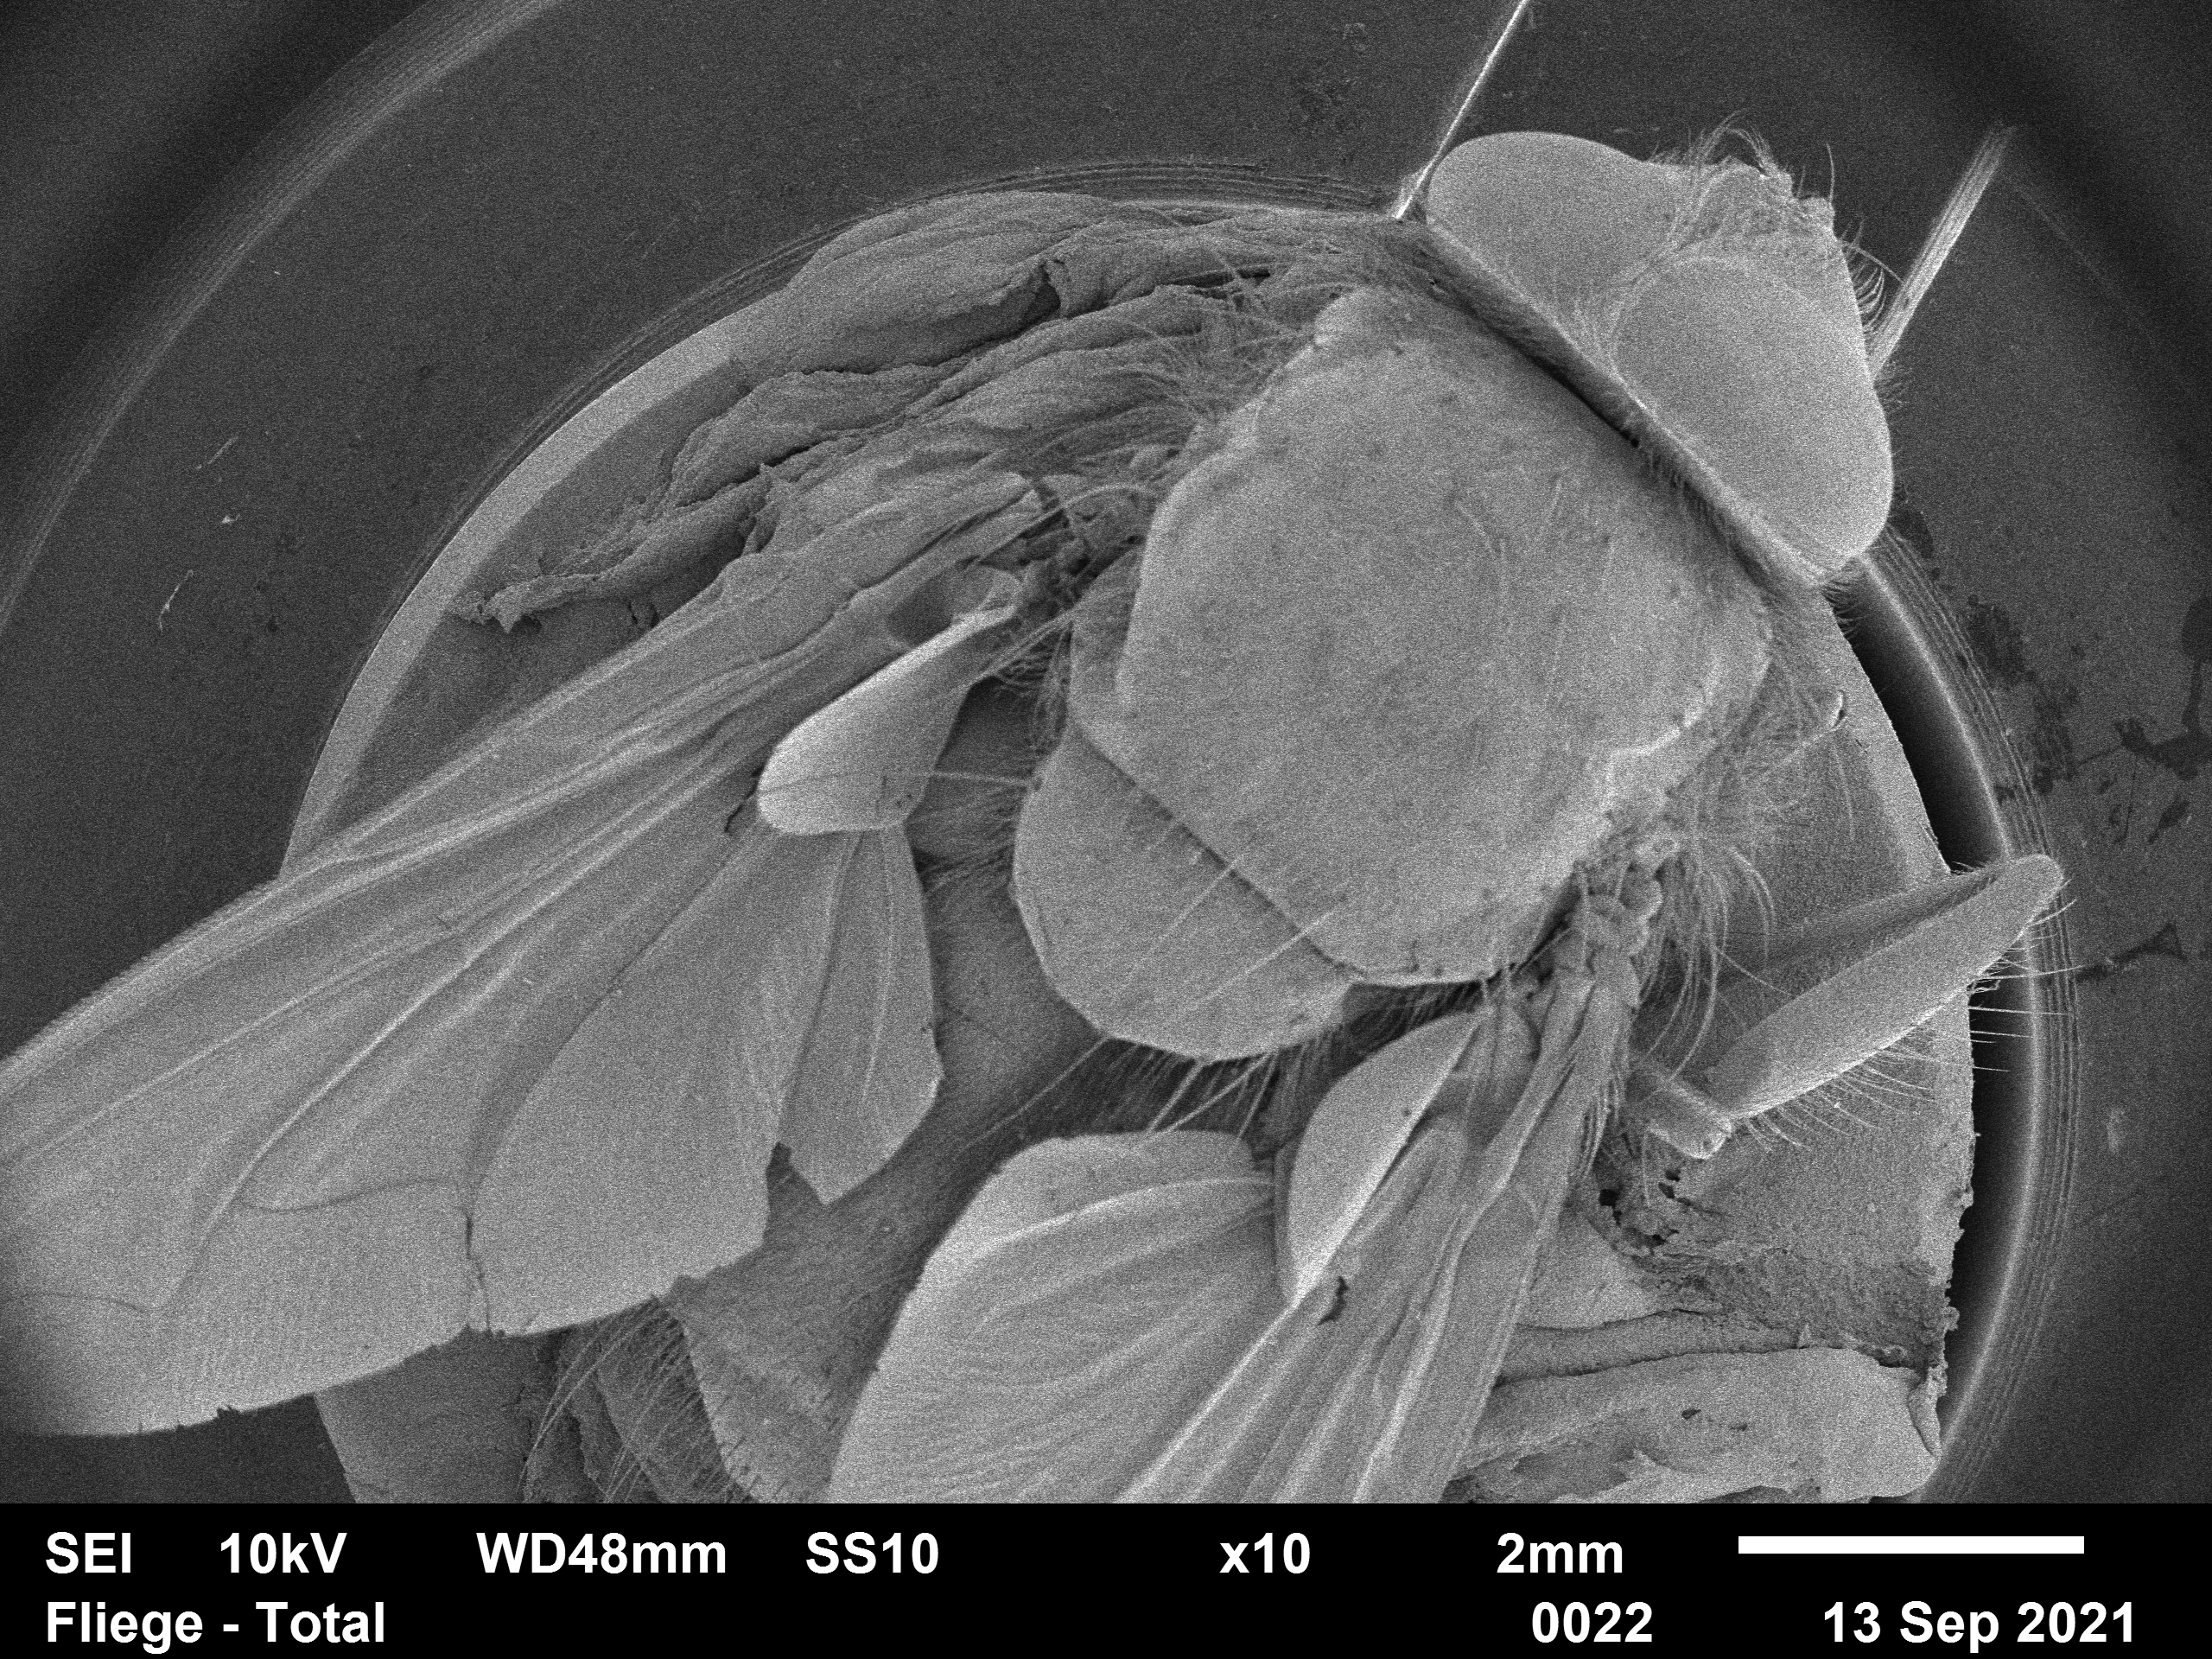
\includegraphics[width=\textwidth]{Auswertung/B/0022.png}
    \caption{Gesamtaufnahme der Fliege}
\end{figure}

\newpage
Als Nächstes wurde ein Segment des Facettenauges vermessen.
\begin{figure}[h]
    \centering
    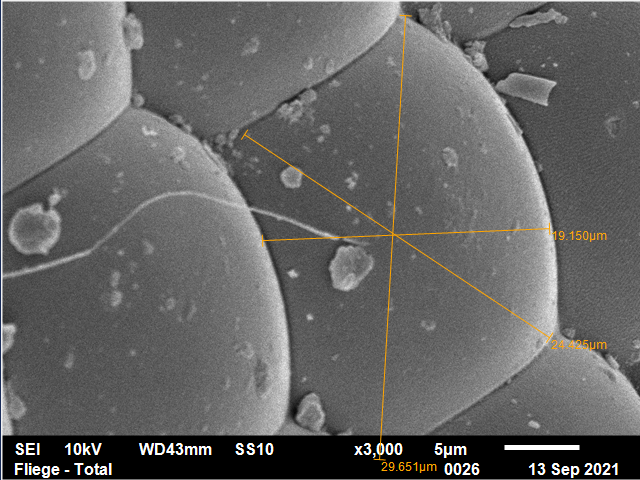
\includegraphics[width=\textwidth]{Auswertung/B/26-2.PNG}
    \caption{Segment eines Facettenauges der Fliege mit Bemaßung}
\end{figure}

Die größe der Segmente beläuft sich auf ca. 20 $\mu$m.

\section{Zinnstandart}


\section{Gebrochene Schraube}


\section{Chip Wafer}